%%%%%%%%%%%%%%%%%%%%%%%%%%%%%%%%%%%%%%%%%
%  My documentation report
%  Objetive: Explain what I did and how, so someone can continue with the investigation
%
% Important note:
% Chapter heading images should have a 2:1 width:height ratio,
% e.g. 920px width and 460px height.
%
%%%%%%%%%%%%%%%%%%%%%%%%%%%%%%%%%%%%%%%%%

%----------------------------------------------------------------------------------------
%	PACKAGES AND OTHER DOCUMENT CONFIGURATIONS
%----------------------------------------------------------------------------------------

\documentclass[11pt,fleqn]{book} % Default font size and left-justified equations

\usepackage[top=3cm,bottom=3cm,left=3.2cm,right=3.2cm,headsep=10pt,letterpaper]{geometry} % Page margins
\usepackage[dvipsnames]{xcolor}
\usepackage{lipsum} % Required for specifying colors by name

% Font Settings
\usepackage{avant} % Use the Avantgarde font for headings
%\usepackage{times} % Use the Times font for headings
\usepackage{mathptmx} % Use the Adobe Times Roman as the default text font together with math symbols from the Symbol, Chancery and Computer Modern fonts

\usepackage{microtype} % Slightly tweak font spacing for aesthetics
\usepackage[utf8]{inputenc} % Required for including letters with accents
\usepackage[T1]{fontenc} % Use 8-bit encoding that has 256 glyphs

%-------- LANGUAGE ------
\usepackage{ifthen}

\provideboolean{lfrench}\setboolean{lfrench}{false} 
\provideboolean{lenglish}\setboolean{lenglish}{false} 

%\setboolean{lfrench}{true} %FRANCAIS
\setboolean{lenglish}{true} % ENGLISH

\ifthenelse{\boolean{lfrench}}{
\usepackage[french]{varioref}
\usepackage[french]{babel}
}{}

\ifthenelse{\boolean{lenglish}}{
\usepackage[english]{varioref}
%\usepackage[english]{babel}
}{}

% ------------------
\usepackage{wrapfig}
\usepackage{listings}
\usepackage{multicol}
\usepackage{multirow}
\usepackage{colortbl}
\usepackage{booktabs}
\newcommand{\tabitem}{~~\llap{\textbullet}~~}
\usepackage[backpage=page]{hyperref}
\usepackage{qrcode}
\usepackage{soul}
\usepackage{tabto}
\usepackage{multienum}

\definecolor{deepblue}{rgb}{0.0,0.0,0.5}
\definecolor{deepred}{rgb}{0.6,0,0}
\definecolor{deepgreen}{rgb}{0,0.5,0}
\definecolor{ocre}{RGB}{51,102,0} 
\definecolor{lightgray}{RGB}{229,229,229} 
\definecolor{palerod}{RGB}{238,232,170}
\definecolor{verttelecom}{RGB}{171,180,0}

\newcommand\pythonstyle{\lstset{
language=Python,
basicstyle=\ttfamily\footnotesize,
morekeywords={self},              % Add keywords here
frame=tb,                         % Any extra options here
showstringspaces=false
}}

\definecolor{backcolour}{rgb}{0.95,0.95,0.92}

\newcommand\termctyle{\lstset{
frame=tb,                         % Any extra options here
showstringspaces=false
}}


% Python environment
\lstnewenvironment{python}[1][]
{
\pythonstyle
\lstset{#1}
}
{}

\lstnewenvironment{termc}[1][]
{
\lstset{#1}
}
{}


% RFC
\newcommand\rfc[1]{\href{http://www.ietf.org/rfc/rfc#1.txt}{\textcolor{blue}{RFC #1}\index{RFC #1}}}
\newcommand\pfunction[2]{\texttt{#2}\index{Module Python!#1!#2}}

% boot.py

\newcommand\glos[1]{\gls{#1}\index{#1}}
\newcommand\pprog[2]{\href{https://github.com/ltn22/PLIDObis/blob/master/#2/#1}{\texttt{#1}}\index{Programmes Python!#1}}
\newcommand\lprog[2]{\href{https://github.com/ltn22/PLIDObis/blob/master/#2/#1}{\texttt{#1}}\index{Programmes micro-python!#1}}

% QUESTION

\usepackage[most]{tcolorbox}

\provideboolean{Response}\setboolean{Response}{true}

\newcommand{\Correct}[1]{\ifthenelse{\boolean{Response}}{#1}{\textbf{#1}}}
\newcommand{\Wrong}[1]{\ifthenelse{\boolean{Response}}{#1}{\textcolor{black!20}{#1}}}

\newwrite\tempfile
\immediate\openout\tempfile=questions.tex


\newtcbtheorem[auto counter,number within=section]{theo}%
  {Question}{fonttitle=\bfseries\upshape, 
     arc=0mm, colback=blue!5!white,colframe=blue!75!black}{Question}
     
\newcommand\Question[3]{
\begin{theo}{#1}{summation}
#2
\immediate\write\tempfile{\noexpand\textbf{Question \thetcbcounter {} page \thepage} {} }
\immediate\write\tempfile{\unexpanded{#2}\noexpand\vspace{1em}\noexpand\newline}
\immediate\write\tempfile{\unexpanded{#3}\noexpand\newline\noexpand\newline}

\end{theo}
}

% MATHS PACKAGE
\usepackage{amsmath,tikz}
\usetikzlibrary{matrix}
\newcommand*{\horzbar}{\rule[0.05ex]{2.5ex}{0.5pt}}
\usepackage{calc}

% VERBATIM PACKAGE
\usepackage{verbatim}

\usepackage{tikz}

\usetikzlibrary{automata}
\usetikzlibrary[shadows]
\usetikzlibrary{shapes}
\usetikzlibrary[decorations.footprints] 
\usetikzlibrary{decorations.pathmorphing}
\usetikzlibrary{decorations.pathreplacing}
\usetikzlibrary{decorations.text}
\usetikzlibrary {arrows}
\usetikzlibrary{patterns}
\usetikzlibrary{calc}
\usetikzlibrary{external}

\usepackage{tikz-timing}

% Acronyms

\usepackage{makeidx}
\makeindex

\usepackage{acronym}

\let\oldac\ac
\renewcommand*{\ac}[1]{\oldac{#1}\index{#1}}

%\usepackage{marginnote}

%\setmarginnotefont{\small\itshape\color{blue}}
\newcommand\Index[1]{\textbf{#1}\index{#1} } %\marginnote{#1} }

% Bibliography
\usepackage[style=alphabetic,sorting=nyt,sortcites=true,autopunct=true,babel=hyphen,hyperref=true,abbreviate=false,backref=true,backend=biber]{biblatex}
\addbibresource{bibliography.bib} % BibTeX bibliography file
\defbibheading{bibempty}{}

%----------------------------------------------------------------------------------------
%	VARIOUS REQUIRED PACKAGES
%----------------------------------------------------------------------------------------

\usepackage{titlesec} % Allows customization of titles

\usepackage{graphicx} % Required for including pictures
\graphicspath{{Pictures/}} % Specifies the directory where pictures are stored

\usepackage{lipsum} % Inserts dummy text

\usepackage{tikz} % Required for drawing custom shapes

\usepackage[french]{babel} % English language/hyphenation

\usepackage{enumitem} % Customize lists
\setlist{nolistsep} % Reduce spacing between bullet points and numbered lists

\usepackage{booktabs} % Required for nicer horizontal rules in tables

\usepackage{eso-pic} % Required for specifying an image background in the title page

%----------------------------------------------------------------------------------------
%	MAIN TABLE OF CONTENTS
%----------------------------------------------------------------------------------------

\usepackage{titletoc} % Required for manipulating the table of contents

\contentsmargin{0cm} % Removes the default margin
% Chapter text styling
\titlecontents{chapter}[1.25cm] % Indentation
{\addvspace{15pt}\large\sffamily\bfseries} % Spacing and font options for chapters
{\color{ocre!60}\contentslabel[\Large\thecontentslabel]{1.25cm}\color{ocre}} % Chapter number
{}  
{\color{ocre!60}\normalsize\sffamily\bfseries\;\titlerule*[.5pc]{.}\;\thecontentspage} % Page number
% Section text styling
\titlecontents{section}[1.25cm] % Indentation
{\addvspace{5pt}\sffamily\bfseries} % Spacing and font options for sections
{\contentslabel[\thecontentslabel]{1.25cm}} % Section number
{}
{\sffamily\hfill\color{black}\thecontentspage} % Page number
[]
% Subsection text styling
\titlecontents{subsection}[1.25cm] % Indentation
{\addvspace{1pt}\sffamily\small} % Spacing and font options for subsections
{\contentslabel[\thecontentslabel]{1.25cm}} % Subsection number
{}
{\sffamily\;\titlerule*[.5pc]{.}\;\thecontentspage} % Page number
[] 

%----------------------------------------------------------------------------------------
%	MINI TABLE OF CONTENTS IN CHAPTER HEADS
%----------------------------------------------------------------------------------------

% Section text styling
\titlecontents{lsection}[0em] % Indendating
{\footnotesize\sffamily} % Font settings
{}
{}
{}

% Subsection text styling
\titlecontents{lsubsection}[.5em] % Indentation
{\normalfont\footnotesize\sffamily} % Font settings
{}
{}
{}
 
%----------------------------------------------------------------------------------------
%	PAGE HEADERS
%----------------------------------------------------------------------------------------

\usepackage{fancyhdr} % Required for header and footer configuration

\pagestyle{fancy}
\renewcommand{\chaptermark}[1]{\markboth{\sffamily\normalsize\bfseries\chaptername\ \thechapter.\ #1}{}} % Chapter text font settings
\renewcommand{\sectionmark}[1]{\markright{\sffamily\normalsize\thesection\hspace{5pt}#1}{}} % Section text font settings
\fancyhf{} \fancyhead[LE,RO]{\sffamily\normalsize\thepage} % Font setting for the page number in the header
\fancyhead[LO]{\rightmark} % Print the nearest section name on the left side of odd pages
\fancyhead[RE]{\leftmark} % Print the current chapter name on the right side of even pages
\renewcommand{\headrulewidth}{0.5pt} % Width of the rule under the header
\addtolength{\headheight}{2.5pt} % Increase the spacing around the header slightly
\renewcommand{\footrulewidth}{0pt} % Removes the rule in the footer
\fancypagestyle{plain}{\fancyhead{}\renewcommand{\headrulewidth}{0pt}} % Style for when a plain pagestyle is specified

% Removes the header from odd empty pages at the end of chapters
\makeatletter
\renewcommand{\cleardoublepage}{
\clearpage\ifodd\c@page\else
\hbox{}
\vspace*{\fill}
\thispagestyle{empty}
\newpage
\fi}

%----------------------------------------------------------------------------------------
%	THEOREM STYLES
%----------------------------------------------------------------------------------------

\usepackage{amsmath,amsfonts,amssymb,amsthm} % For math equations, theorems, symbols, etc

\newcommand{\intoo}[2]{\mathopen{]}#1\,;#2\mathclose{[}}
\newcommand{\ud}{\mathop{\mathrm{{}d}}\mathopen{}}
\newcommand{\intff}[2]{\mathopen{[}#1\,;#2\mathclose{]}}
\newtheorem{notation}{Notation}[chapter]

%%%%%%%%%%%%%%%%%%%%%%%%%%%%%%%%%%%%%%%%%%%%%%%%%%%%%%%%%%%%%%%%%%%%%%%%%%%
%%%%%%%%%%%%%%%%%%%% dedicated to boxed/framed environements %%%%%%%%%%%%%%
%%%%%%%%%%%%%%%%%%%%%%%%%%%%%%%%%%%%%%%%%%%%%%%%%%%%%%%%%%%%%%%%%%%%%%%%%%%
\newtheoremstyle{ocrenumbox}% % Theorem style name
{0pt}% Space above
{0pt}% Space below
{\normalfont}% % Body font
{}% Indent amount
{\small\bf\sffamily\color{ocre}}% % Theorem head font
{\;}% Punctuation after theorem head
{0.25em}% Space after theorem head
{\small\sffamily\color{ocre}\thmname{#1}\nobreakspace\thmnumber{\@ifnotempty{#1}{}\@upn{#2}}% Theorem text (e.g. Theorem 2.1)
\thmnote{\nobreakspace\the\thm@notefont\sffamily\bfseries\color{black}---\nobreakspace#3.}} % Optional theorem note
\renewcommand{\qedsymbol}{$\blacksquare$}% Optional qed square

\newtheoremstyle{blacknumex}% Theorem style name
{5pt}% Space above
{5pt}% Space below
{\normalfont}% Body font
{} % Indent amount
{\small\bf\sffamily}% Theorem head font
{\;}% Punctuation after theorem head
{0.25em}% Space after theorem head
{\small\sffamily{\tiny\ensuremath{\blacksquare}}\nobreakspace\thmname{#1}\nobreakspace\thmnumber{\@ifnotempty{#1}{}\@upn{#2}}% Theorem text (e.g. Theorem 2.1)
\thmnote{\nobreakspace\the\thm@notefont\sffamily\bfseries---\nobreakspace#3.}}% Optional theorem note

\newtheoremstyle{blacknumbox} % Theorem style name
{0pt}% Space above
{0pt}% Space below
{\normalfont}% Body font
{}% Indent amount
{\small\bf\sffamily}% Theorem head font
{\;}% Punctuation after theorem head
{0.25em}% Space after theorem head
{\small\sffamily\thmname{#1}\nobreakspace\thmnumber{\@ifnotempty{#1}{}\@upn{#2}}% Theorem text (e.g. Theorem 2.1)
\thmnote{\nobreakspace\the\thm@notefont\sffamily\bfseries---\nobreakspace#3.}}% Optional theorem note

%%%%%%%%%%%%%%%%%%%%%%%%%%%%%%%%%%%%%%%%%%%%%%%%%%%%%%%%%%%%%%%%%%%%%%%%%%%
%%%%%%%%%%%%% dedicated to non-boxed/non-framed environements %%%%%%%%%%%%%
%%%%%%%%%%%%%%%%%%%%%%%%%%%%%%%%%%%%%%%%%%%%%%%%%%%%%%%%%%%%%%%%%%%%%%%%%%%
\newtheoremstyle{ocrenum}% % Theorem style name
{5pt}% Space above
{5pt}% Space below
{\normalfont}% % Body font
{}% Indent amount
{\small\bf\sffamily\color{ocre}}% % Theorem head font
{\;}% Punctuation after theorem head
{0.25em}% Space after theorem head
{\small\sffamily\color{ocre}\thmname{#1}\nobreakspace\thmnumber{\@ifnotempty{#1}{}\@upn{#2}}% Theorem text (e.g. Theorem 2.1)
\thmnote{\nobreakspace\the\thm@notefont\sffamily\bfseries\color{black}---\nobreakspace#3.}} % Optional theorem note
\renewcommand{\qedsymbol}{$\blacksquare$}% Optional qed square
\makeatother

% Defines the theorem text style for each type of theorem to one of the three styles above
\newcounter{dummy} 
\numberwithin{dummy}{section}
\theoremstyle{ocrenumbox}
\newtheorem{theoremeT}[dummy]{Theorem}
\newtheorem{problem}{Problem}[chapter]
\newtheorem{exerciseT}{Exercise}[chapter]
\theoremstyle{blacknumex}
\newtheorem{exampleT}{Example}[chapter]
\theoremstyle{blacknumbox}
\newtheorem{vocabulary}{Vocabulary}[chapter]
\newtheorem{definitionT}{Definition}[section]
\newtheorem{corollaryT}[dummy]{Corollary}
\theoremstyle{ocrenum}
\newtheorem{proposition}[dummy]{Proposition}

%----------------------------------------------------------------------------------------
%	DEFINITION OF COLORED BOXES
%----------------------------------------------------------------------------------------

\RequirePackage[framemethod=default]{mdframed} % Required for creating the theorem, definition, exercise and corollary boxes

% Theorem box
\newmdenv[skipabove=7pt,
skipbelow=7pt,
backgroundcolor=black!5,
linecolor=ocre,
innerleftmargin=5pt,
innerrightmargin=5pt,
innertopmargin=5pt,
leftmargin=0cm,
rightmargin=0cm,
innerbottommargin=5pt]{tBox}

% Exercise box	  
\newmdenv[skipabove=7pt,
skipbelow=7pt,
rightline=false,
leftline=true,
topline=false,
bottomline=false,
backgroundcolor=ocre!10,
linecolor=ocre,
innerleftmargin=5pt,
innerrightmargin=5pt,
innertopmargin=5pt,
innerbottommargin=5pt,
leftmargin=0cm,
rightmargin=0cm,
linewidth=4pt]{eBox}	

% Definition box
\newmdenv[skipabove=7pt,
skipbelow=7pt,
rightline=false,
leftline=true,
topline=false,
bottomline=false,
linecolor=ocre,
innerleftmargin=5pt,
innerrightmargin=5pt,
innertopmargin=0pt,
leftmargin=0cm,
rightmargin=0cm,
linewidth=4pt,
innerbottommargin=0pt]{dBox}	

% Corollary box
\newmdenv[skipabove=7pt,
skipbelow=7pt,
rightline=false,
leftline=true,
topline=false,
bottomline=false,
linecolor=gray,
backgroundcolor=black!5,
innerleftmargin=5pt,
innerrightmargin=5pt,
innertopmargin=5pt,
leftmargin=0cm,
rightmargin=0cm,
linewidth=4pt,
innerbottommargin=5pt]{cBox}

% Creates an environment for each type of theorem and assigns it a theorem text style from the "Theorem Styles" section above and a colored box from above
\newenvironment{theorem}{\begin{tBox}\begin{theoremeT}}{\end{theoremeT}\end{tBox}}
\newenvironment{exercise}{\begin{eBox}\begin{exerciseT}}{\hfill{\color{ocre}\tiny\ensuremath{\blacksquare}}\end{exerciseT}\end{eBox}}				  
\newenvironment{definition}{\begin{dBox}\begin{definitionT}}{\end{definitionT}\end{dBox}}	
\newenvironment{example}{\begin{exampleT}}{\hfill{\tiny\ensuremath{\blacksquare}}\end{exampleT}}		
\newenvironment{corollary}{\begin{cBox}\begin{corollaryT}}{\end{corollaryT}\end{cBox}}	

%----------------------------------------------------------------------------------------
%	REMARK ENVIRONMENT
%----------------------------------------------------------------------------------------

\newenvironment{remark}{\par\vspace{10pt}\small % Vertical white space above the remark and smaller font size
\begin{list}{}{
\leftmargin=35pt % Indentation on the left
\rightmargin=25pt}\item\ignorespaces % Indentation on the right
\makebox[-2.5pt]{\begin{tikzpicture}[overlay]
\node[draw=ocre!60,line width=1pt,circle,fill=ocre!25,font=\sffamily\bfseries,inner sep=2pt,outer sep=0pt] at (-15pt,0pt){\textcolor{ocre}{R}};\end{tikzpicture}} % Orange R in a circle
\advance\baselineskip -1pt}{\end{list}\vskip5pt} % Tighter line spacing and white space after remark

%----------------------------------------------------------------------------------------
%	SECTION NUMBERING IN THE MARGIN
%----------------------------------------------------------------------------------------

\makeatletter
\renewcommand{\@seccntformat}[1]{\llap{\textcolor{ocre}{\csname the#1\endcsname}\hspace{1em}}}                    
\renewcommand{\section}{\@startsection{section}{1}{\z@}
{-4ex \@plus -1ex \@minus -.4ex}
{1ex \@plus.2ex }
{\normalfont\large\sffamily\bfseries}}
\renewcommand{\subsection}{\@startsection {subsection}{2}{\z@}
{-3ex \@plus -0.1ex \@minus -.4ex}
{0.5ex \@plus.2ex }
{\normalfont\sffamily\bfseries}}
\renewcommand{\subsubsection}{\@startsection {subsubsection}{3}{\z@}
{-2ex \@plus -0.1ex \@minus -.2ex}
{.2ex \@plus.2ex }
{\normalfont\small\sffamily\bfseries}}                        
\renewcommand\paragraph{\@startsection{paragraph}{4}{\z@}
{-2ex \@plus-.2ex \@minus .2ex}
{.1ex}
{\normalfont\small\sffamily\bfseries}}

%----------------------------------------------------------------------------------------
%	HYPERLINKS IN THE DOCUMENTS
%----------------------------------------------------------------------------------------

% For an unclear reason, the package should be loaded now and not later
\usepackage{hyperref}
\hypersetup{hidelinks,backref=true,pagebackref=true,hyperindex=true,colorlinks=false,breaklinks=true,urlcolor= ocre,bookmarks=true,bookmarksopen=false,pdftitle={Title},pdfauthor={Author}}

%----------------------------------------------------------------------------------------
%	CHAPTER HEADINGS
%----------------------------------------------------------------------------------------

% The set-up below should be (sadly) manually adapted to the overall margin page septup controlled by the geometry package loaded in the main.tex document. It is possible to implement below the dimensions used in the goemetry package (top,bottom,left,right)... TO BE DONE

\newcommand{\thechapterimage}{}
\newcommand{\chapterimage}[1]{\renewcommand{\thechapterimage}{#1}}

% Numbered chapters with mini tableofcontents
\def\thechapter{\arabic{chapter}}
\def\@makechapterhead#1{
\thispagestyle{empty}
{\centering \normalfont\sffamily
\ifnum \c@secnumdepth >\m@ne
\if@mainmatter
\startcontents
\begin{tikzpicture}[remember picture,overlay]
\node at (current page.north west)
{\begin{tikzpicture}[remember picture,overlay]
\node[anchor=north west,inner sep=0pt] at (0,0) {\includegraphics[width=\paperwidth]{\thechapterimage}};
%%%%%%%%%%%%%%%%%%%%%%%%%%%%%%%%%%%%%%%%%%%%%%%%%%%%%%%%%%%%%%%%%%%%%%%%%%%%%%%%%%%%%
% Commenting the 3 lines below removes the small contents box in the chapter heading
%\fill[color=ocre!10!white,opacity=.6] (1cm,0) rectangle (8cm,-7cm);
%\node[anchor=north west] at (1.1cm,.35cm) {\parbox[t][8cm][t]{6.5cm}{\huge\bfseries\flushleft \printcontents{l}{1}{\setcounter{tocdepth}{2}}}};
\draw[anchor=west] (5cm,-9cm) node [rounded corners=20pt,fill=ocre!10!white,text opacity=1,draw=ocre,draw opacity=1,line width=1.5pt,fill opacity=.6,inner sep=12pt]{\huge\sffamily\bfseries\textcolor{black}{\thechapter. #1\strut\makebox[22cm]{}}};
%%%%%%%%%%%%%%%%%%%%%%%%%%%%%%%%%%%%%%%%%%%%%%%%%%%%%%%%%%%%%%%%%%%%%%%%%%%%%%%%%%%%%
\end{tikzpicture}};
\end{tikzpicture}}
\par\vspace*{230\p@}
\fi
\fi}

% Unnumbered chapters without mini tableofcontents (could be added though) 
\def\@makeschapterhead#1{
\thispagestyle{empty}
{\centering \normalfont\sffamily
\ifnum \c@secnumdepth >\m@ne
\if@mainmatter
\begin{tikzpicture}[remember picture,overlay]
\node at (current page.north west)
{\begin{tikzpicture}[remember picture,overlay]
\node[anchor=north west,inner sep=0pt] at (0,0) {\includegraphics[width=\paperwidth]{\thechapterimage}};
\draw[anchor=west] (5cm,-9cm) node [rounded corners=20pt,fill=ocre!10!white,fill opacity=.6,inner sep=12pt,text opacity=1,draw=ocre,draw opacity=1,line width=1.5pt]{\huge\sffamily\bfseries\textcolor{black}{#1\strut\makebox[22cm]{}}};
\end{tikzpicture}};
\end{tikzpicture}}
\par\vspace*{230\p@}
\fi
\fi
}
\makeatother % Insert the commands.tex file which contains the majority of the structure behind the template



\newcommand\pythonlst[2][]{
\lstinputlisting[language=Python, backgroundcolor=\color{palerod},   basicstyle=\footnotesize\ttfamily,
  keywordstyle=\bfseries\color{green!40!black},
  commentstyle=\itshape\color{purple!40!black},
  identifierstyle=\color{blue},
  stringstyle=\color{orange}, caption=#2,
  numbers=left, numberstyle=\tiny, stepnumber=2, numbersep=5pt, frame=single, #1] {Programs/#2}\index{Programmes Python!#2}
  }

\newcommand\pythonnxt[2][]{
\lstinputlisting[language=Python, backgroundcolor=\color{palerod},   basicstyle=\footnotesize\ttfamily,
  keywordstyle=\bfseries\color{green!40!black},
  commentstyle=\itshape\color{purple!40!black},
  identifierstyle=\color{blue},
  stringstyle=\color{orange},
  numbers=left, numberstyle=\tiny, stepnumber=2, numbersep=5pt, frame=single, #1] {Programs/#2}
  }
  
  
\newcommand\pycomlst[2][]{
\lstinputlisting[language=Python, backgroundcolor=\color{gray!10},   basicstyle=\footnotesize\ttfamily,
  keywordstyle=\bfseries\color{green!40!black},
  commentstyle=\itshape\color{purple!40!black},
  identifierstyle=\color{blue},
  stringstyle=\color{orange}, caption=#2,
  numbers=left, numberstyle=\tiny, stepnumber=2, numbersep=5pt, frame=single, #1] {Programs/#2}\index{Programmes micro-python!#2}
  }

\newcommand\pycomnxt[2][]{
\lstinputlisting[language=Python, backgroundcolor=\color{gray!10},   basicstyle=\footnotesize\ttfamily,
  keywordstyle=\bfseries\color{green!40!black},
  commentstyle=\itshape\color{purple!40!black},
  identifierstyle=\color{blue},
  stringstyle=\color{orange},
  numbers=left, numberstyle=\tiny, stepnumber=2, numbersep=5pt, frame=single, #1] {Programs/#2}
  }



\newcommand\Youtube[1]{\begin{tcolorbox}[colback=red!5,colframe=red!75!black,title=Youtube, width=3cm]\href{#1}{\qrcode{#1}}\end{tcolorbox}}

\newcommand\fulluri[2]{\href{#2}{#1}\footnote{\url{#2}}}
%%%%%%%

\provideboolean{allchap}\setboolean{allchap}{false}

\newcommand\Input[1]{\ifthenelse{\boolean{allchap}}{\input{#1}}{}}


%-----------



\newcommand\lgf[1]{\ifthenelse{\boolean{lfrench}}{#1}{}}%
\newcommand\lge[1]{\ifthenelse{\boolean{lenglish}}{#1}{}}%

\newcommand\Vrai[0]{\ifthenelse{\boolean{lfrench}}{Vrai}{}\ifthenelse{\boolean{lenglish}}{True}{}}
\newcommand\Faux[0]{\ifthenelse{\boolean{lfrench}}{Faux}{}\ifthenelse{\boolean{lenglish}}{False}{}}

\documentclass{article}

\ifthenelse{\boolean{lfrench}}{
\usepackage[
    type={CC},
    modifier={by-nc-nd},
    version={3.0},
]{doclicense}
} { % by default in english
\usepackage[
    type={CC},
    modifier={by-nc-nd},
    version={3.0},
    lang=English,
]{doclicense}
}


\begin{document}

\let\cleardoublepage\clearpage

%----------------------------------------------------------------------------------------
%	TITLE PAGE
%----------------------------------------------------------------------------------------

\begingroup
\thispagestyle{empty}
\AddToShipoutPicture*{\put(0,0){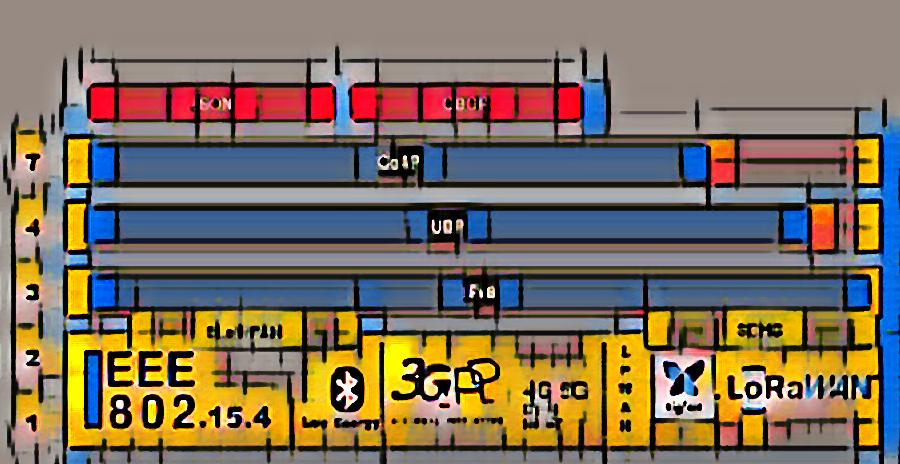
\includegraphics[scale=.70]{Pictures/cover.jpeg}}} % Image background
\centering
\vspace*{5cm}
\par\normalfont\fontsize{35}{35}\sffamily\selectfont
\lgf{\textbf{PROGRAMMER L'INTERNET DES OBJETS }}
\lge{\textbf{PROGRAMMING THE INTERNET OF THINGS }}
{\LARGE }\par % Book title
\vspace*{1cm}
{\Huge Laurent TOUTAIN}\par % Author name
\endgroup

%----------------------------------------------------------------------------------------
%	COPYRIGHT PAGE
%----------------------------------------------------------------------------------------

\newpage
~\vfill
\thispagestyle{empty}

%\noindent Copyright \copyright\ 2014 Andrea Hidalgo\\ % Copyright notice

\noindent \textsc{IMT Atlantique}\\
\doclicenseThis

\noindent \lgf{Basé sur le \href{https://bit.ly/3Ku0aL8}{MOOC PLIDO}.}\\ % License information
\lge{Based on the  \href{https://bit.ly/3Ku0aL8}{PLIDO MOOC}.} \\
\noindent \textit{\lgf{Publié le \today}\lge{Published \today}} % Printing/edition date

%----------------------------------------------------------------------------------------
%	TABLE OF CONTENTS
%----------------------------------------------------------------------------------------


\chapterimage{pano-tv1.png} % Chapter heading image

\pagestyle{empty} % No headers

\ifthenelse{\boolean{lfrench}}{
\renewcommand\contentsname{Table des Matières}
\renewcommand{\bibname}{Bibliographie}
}{}
\ifthenelse{\boolean{lenglish}}{
\renewcommand\contentsname{Table of Contents}
\renewcommand{\bibname}{Bibliography}
}{}

\cleardoublepage
\tableofcontents% Print the table of contents itself

%\cleardoublepage % Forces the first chapter to start on an odd page so it's on the right

\pagestyle{fancy} % Print headers again

%----------------------------------------------------------------------------------------
%	CHAPTERS
%----------------------------------------------------------------------------------------
\cleardoublepage

\lgf{\chapter*{Acronymes}}
\lge{\chapter*{Acronyms}}

\begin{multicols}{2}
\begin{acronym}
\acro{3GPP}{3rd Generation Partnership Project}
\acro{ABP}{Authentication By Personalisation}
\acro{ADSL}{Asymmetric Digital Subscriber Line}
\acro{AMQP}{Advanced Message Queuing Protocol}
\acro{AS}{Application Server}
\acro{ASCII}{American Standard Code for Information Interchange}
\acro{BLE}{Bluetooth Low Energy}
\acro{CBOR}{Concise Binaire Object Representation}
\acro{CoAP}{Constrained Application Protocol}
\acro{Cosem}{Companion Specification for Energy Management}
\acro{CRC}{Cyclic Redundancy Check}
\acro{CSV}{Comma Separated Values}
\acro{DLMS}{Device Language Message Specification}
\acro{DTT}{Digital Terrestrial Television}
\acro{DR}{Data Rate}
\acro{GSMA}{GSM Association}
\acro{HTML}{HyperText Markup Language}
\acro{HTTP}{HyperText Transport Protocol}
\acro{HTTPS}{HyperText Transport Protocol Secure}
\acro{IANA}{Internet Assigned Numbers Authority}
\acro{IBAN}{International Bank Account Number}
\acro{IEEE}{Institute of Electrical and Electronics Engineers}
\acro{IETF}{Internet Engineering Task Force}
\acro{IoT}{Internet of Things}
\acro{IP}{Internet Protocol}
\acro{IPv4}{Internet Protocol version 4}
\acro{IPv6}{Internet Protocol version 6}
\acro{IPSO}{IP for Smart Objects}
\acro{ITU}{International Telecommunication Union}
\acro{IRI}{International Resource Identifier}
\acro{ISBN}{International Standard Book Number}
\acro{ISO}{International Standardization Organization}
\acro{JMS}{Java Messaging Service}
\acro{JSON}{JavaScript Object Notation}
\acro{JSON-LD}{JavaScript Object Notation  for Linked Data}
\acro{LCIM}{Levels of Conceptual Interoperability Model}
\acro{LPWAN}{Low Power Wide Area Network}
\acro{LwM2M}{Lightweight Machine to Machine}
\acro{LNS}{LoRaWAN Network Server}
\acro{MQTT}{Message Queuing Telemetry Transport}
\acro{NAT}{Network Address Translation}
\acro{NGW}{Network GateWay}
\acro{NIDD}{Non IP Data Delivery}
\acro{OMA}{Open Mobile Alliance}
\acro{OTAA}{Over The Air Authentication}
\acro{OVH}{On Vous Herbèrge}
\acro{PAC}{Porting Authorization Code}
\acro{REST}{REpresentational State Transfer}
\acro{RFC}{Request For Comments}
\acro{RGW}{Radio GateWay}
\acro{RNIPP}{Répertoire National d'Identification des Personnes Physiques}
\acro{RSSI}{Received Signal Strength Indicator}
\acro{RTT}{Round Trip Time}
\acro{SCEF}{Service Capability Exposure Function}
\acro{SenML}{Sensor Measuring List}
\acro{SCHC}{Static Context Header Compression}
\acro{SF}{Spreading Factor}
\acro{SNR}{Signal to Noise Ratio}
\acro{SSID}{Service Set IDentifier}
\acro{STIC}{Sciences et Technologies de l’Information et de la Communication}
\acro{TCP}{Transmission Control Protocol}
\acro{TLV}{Type Length Value}
\acro{TNT}{Télévision Numérique Terrestre}
\acro{TTN}{The Things Network}
\acro{UDP}{User Datagram Protocol}
\acro{UIT}{Union internationale des télécommunications}
\acro{UNB}{Ultra Narrow-Band}
\acro{URI}{Universal Resource Identifier}
\acro{URL}{Univeral Resource Locator}
\acro{URN}{Univeral Resource Name}
\acro{VPS}{Virtual Private Server}
\acro{W3C}{World Wide Web Consortium}
\acro{WWW}{World Wide Web}
\acro{XML}{Extensible Markup Language}
\acro{XMPP}{Extensible Messaging Protocol et Presence}
\end{acronym}
\end{multicols}

%\setboolean{allchap}{true} % true: take all, false take nothing only /input



\Input{Part00-liminaire}
\Input{Part01.0-Intro}
\Input{Part02.0-ArchiIP}
\Input{Part02.5-Wireshark}
\Input{Part03.0-Modbus}
\Input{Part04.0-ArchiIoT}
\Input{Part05.0-Data}
\Input{Part06.0-VSensors}
\Input{Part06.5-beebotte}
\Input{Part07.0-LoPy}
\Input{Part08.0-Sigfox}
\Input{Part09.0-LoRaWAN}
\Input{Part10.0-CoAP}
\cleardoublepage
\lgf{\chapter{Experimentons CoAP}}
\lge{\chapter{Let's experiment CoAP}}

\lgf{Les programmes se trouvent dans le répertoire \texttt{pycom} pour l'Objet et \texttt{plido-tp4} pour le serveur.}
\lge{The programs are located in the directory \texttt{pycom} for the Object and \texttt{plido-tp4} for the server.}


\lgf{Les programmes pour l'Objet pourront tourner indifféremment dans une fenêtre de votre ordinateur ou sur votre Pycom. Dans la suite, nous supposerons qu'il s'agit d'une deuxième fenêtre de terminal sur votre ordinateur mais libre à vous de le lancer sur votre Pycom en Wi-Fi (voire en LoRaWAN) pour plus de réalisme. L'utilisation du réseau Sigfox est plus problématique vu que les requêtes provenant de votre Pycom sont limitées à 12 caractères et que les réponses ne sont qu'au nombre de 4 par jour et limitées à 8 caractères. }
\lge{The programs for the Object can run either in a window on your computer or on your Pycom. In the following, we will assume that it is a second terminal window on your computer but feel free to run it on your Pycom in Wi-Fi (or even in LoRaWAN) for more realism. The use of the Sigfox network is more problematic since the requests from your Pycom are limited to 12 characters and the answers are only 4 per day and limited to 8 characters. }

\lgf{Pour nous concentrer sur le fonctionnement de CoAP, nous allons tout d'abord expérimenter en local sur notre ordinateur. Nous verrons par la suite comment utiliser le programme \pprog{generic\_relay.py}{plido-tp3}  pour bénéficier des réseaux LPWAN.}
\lge{To concentrate on the functioning of CoAP, we will first experiment locally on our computer. We will then see how to use the program \pprog{generic\_relay.py}{plido-tp3} to benefit from LPWAN networks}.


\lgf{Attention, le serveur ne fonctionne pas directement sous Windows. Vous devez impérativement le faire tourner dans la machine virtuelle.}
\lge{Be careful, the server does not work directly under Windows. You must run it in the virtual machine.}

\lgf{\section{Mise en œuvre du client/serveur}}
\lge{\section{Client/server implementation}}



 \begin{wrapfigure}{r}{3cm}
\Youtube{https://youtu.be/Nieitr19VGg}
\end{wrapfigure}

\lgf{Nous allons mettre en œuvre le protocole CoAP entre deux processus sur votre machine puis, si vous le voulez, vous pourrez le tester sur un LoPy. Côté Objet, nous allons utiliser une mise en œuvre simple mais compacte du protocole pour comprendre son fonctionnement. À l’autre extrémité, nous utiliserons la mise en œuvre \Index{aiocoap} qui est très complète mais beaucoup plus complexe et demandant plus de ressources.}
\lge{We will implement the CoAP protocol between two processes on your machine and then, if you want, you can test it on a LoPy. On the Object side, we will use a simple but compact implementation of the protocol to understand how it works. At the other end, we will use the \Index{aiocoap} implementation which is very complete but much more complex and resource intensive.}

\subsection{aiocoap}

\lgf{Comme son nom l'indique, aiocoap met en œuvre CoAP, avec les modules asynchronous Input/Output, permettant un fort degré de parallélisme. Le programme suivant (\pprog{coap\_basic\_server1.py}{plido-tp4}) donne un exemple d’un serveur simple gérant une seule ressource time :}
\lge{As its name indicates, aiocoap implements CoAP, with asynchronous Input/Output modules, allowing a high degree of parallelism. The following program (\pprog{coap\_basic\_server1.py}{plido-tp4}) gives an example of a simple server managing a single time resource:}


\pythonlst{coap\_basic\_server1.py}

\begin{itemize}
    \item 
        \lgf{Lignes 21 et 22, l’utilisation de \textit{aicoap} se traduit par l’importation des modules qui se trouvent dans le répertoire \texttt{aoicoap}. }
        \lge{Lines 21 and 22, the use of \textit{aicoap} results in the import of the modules which are in the \texttt{aoicoap} directory. }
    \item  
        \lgf{Dans la fonction \texttt{main} le programme~:}
        \lge{In the function \texttt{main} the program:}
    \begin{itemize}
        \item  
           \lgf{cherche son adresse IP fixe (lignes 40 à 42)~;}
           \lge{looks for its fixed IP address (lines 40 to 42);}
        \item   
            \lgf{fixe à la valeur par défaut le numéro de port à la valeur affectée au serveur CoAP (ligne 44)\footnote{L’utilisation d’une adresse IP et non du joker 0.0.0.0 permet de faire tourner le serveur dans un environnement Windows et MAC};}
            \lge{sets the port number to the default value assigned to the CoAP server (line 44)\footnote{The use of an IP address and not the wildcard 0.0.0.0 allows the server to run in a Windows and MAC environment};}
        \item  
             \lgf{ligne 47, La variable \texttt{root} contient l’arbre des ressources. À la ligne suivante, la ressource \texttt{time} est associée à une classe \texttt{TimeResource}.}
             \lge{line 47, the variable \texttt{root} contains the tree of resources. On the next line, the resource \texttt{time} is associated with a class \texttt{TimeResource}.}
        \item  
        \lgf{La méthode~:}
        \lge{The method:}

\begin{termc}[backgroundcolor=\color{palerod}, basicstyle=\ttfamily\tiny, escapechar=@] 
asyncio.Task(aiocoap.Context.create_server_context(root, bind=(ip_addr, port)))
\end{termc}

            \lgf{permet de lier cet arbre de ressource à l’adresse IP et au numéro de port précédemment défini.}
            \lge{allows to link this resource tree to the IP address and port number previously defined.}
        
        \item  
            \lgf{Ligne 55, le serveur est ensuite lancé dans une boucle sans fin.}
            \lge{Line 55, the server is then launched in an endless loop.}
    \end{itemize}

\end{itemize}

         \vspace{1em}


\lgf{Il est plus intéressant de voir le traitement effectué lorsque la ressource est appelée par le serveur. La classe \texttt{TimeResource} dérivant de la classe générique \texttt{aiocoap} \pfunction{aiocoap}{Resource} est utilisée (ligne 24)~:}
\lge{It is more interesting to see the processing done when the resource is called by the server. The class \texttt{TimeResource} derived from the generic class \texttt{aiocoap} \pfunction{aiocoap}{Resource} is used (line 24):}

\begin{termc}[backgroundcolor=\color{palerod}, basicstyle=\ttfamily\small, escapechar=@] 
class TimeResource(resource.Resource):
\end{termc}

\lgf{Pour chaque méthode CoAP, une méthode peut être définie dans cette classe. Dans l’exemple, la méthode \texttt{render\_get} permet de traiter les requêtes GET. }
\lge{For each CoAP method, a method can be defined in this class. In the example, the method \texttt{render\_get} allows to treat the GET requests. }


         \vspace{1em}


\lgf{Pour simuler un temps de traitement, le programme commence par attendre 5 secondes (ligne 27) puis construit la chaîne de caractères contenant la date qu’il va retourner dans un objet \texttt{aoicoap} \pfunction{aoicoap}{Message}.}
\lge{To simulate a processing time, the program starts by waiting for 5 seconds (line 27) and then constructs the string containing the date that it will return in a \texttt{aoicoap} object \pfunction{aoicoap}{Message}.}

         \vspace{1em}


\lgf{Ainsi, si tout se passe correctement, la réponse à une requête (Code = 0x01) sera 2.05 (Content). La figure~\vref{fig-CoAP-date} résume cet échange que nous avions vu théoriquement dans le chapitre~\vref{chap-token} consacré aux tokens.}
\lge{Thus, if everything goes well, the answer to a request (Code = 0x01) will be 2.05 (Content). The figure~\vref{fig-CoAP-date} summarizes this exchange that we had seen theoretically in the chapter~\vref{chap-token} devoted to tokens.}


\begin{figure}
\centering
	\begin{tikzpicture}[scale=1.5, transform shape] 
	
	\draw [drop shadow, color=verttelecom, -fast cap, line width=3pt] (1, 6) coordinate (a) -- (1, 1);
	\draw [drop shadow, color=verttelecom, -fast cap, line width=3pt] (4, 6) coordinate (b) -- (4, 1);
	
	\draw (a) node [above, verttelecom] {\tiny{Client}};
	\draw (b) node [above, verttelecom] {\tiny{Serveur}};
	
		\draw [ultra thick,  color=purple, drop shadow, ->] (1, 5.5) -- node [above, near end, sloped, text width=4cm] {\tiny{CON MID=0x1234\\Token=12\\GET /time\\}} (4, 5); 
		\draw [color=verttelecom, thick] (1, 5.5) -- +(-0.5, 0); 
		\draw [ultra thick,  color=purple, drop shadow, ->] (4, 5) -- node [below, sloped] {\tiny{ACK MID=0x1234}} (1, 4.5); 
		\draw [color=red, -diamond] (0.75, 5.5) -- node [below, sloped] {\tiny{Timer}} +(0, -1); 
		\draw [color=verttelecom, thick] (1, 4.5) -- +(-0.5, 0); 
		\draw [dotted, color=purple, -triangle 60] (4,5) to [bend left=90] (4, 2.5); 
		\draw [ultra thick,  color=purple, drop shadow, ->] (4, 2.5) -- node [above, near start, sloped, text width=4cm] {\tiny{CON MID=0xF00D\\Token=12\\2.05 "2020-09-05 20:15"\\}} (1, 2); 
		\draw [color=verttelecom, thick] (4, 2.5) -- +(0.5, 0); 
		\draw [ultra thick,  color=purple, drop shadow, ->] (1, 2) -- node [below, sloped] {\tiny{ACK MID=0xF00D}} (4, 1.5); 
		\draw [color=red, -diamond] (4.25, 2.5) -- node [above, sloped] {\tiny{Timer}} +(0, -1); 
		\draw [color=verttelecom, thick] (4, 1.5) -- +(0.5, 0); 
	
	\end{tikzpicture}
\lgf{\caption{Récupération de la date} }
\lge{\caption{Date retrieval} }
\label{fig-CoAP-date} 
\end{figure} 	

\lgf{\subsection{côté Objet}}
\lge{\subsection{Object side}}

\lgf{Du coté du client, nous allons utiliser une mise en œuvre plus compacte qui nous permettra d’expérimenter le fonctionnement de CoAP en modifiant les valeurs des champs protocolaires.}
\lge{On the client side, we will use a more compact implementation that will allow us to experiment the operation of CoAP by changing the values of the protocol fields.}


         \vspace{1em}

\pycomlst{coap\_empty\_msg.py}

\lgf{Le programme \lprog{coap\_empty\_msg.py}{pycom} est beaucoup plus simple. Dans un premier temps, vous devez remplacer l’adresse IP par celle fournie par votre serveur CoAP. Le programme crée une socket UDP au travers de laquelle l’échange avec le serveur sera effectué. La première action consiste à créer un message \lfunction{CoAP}{CoAP} (ligne 9) et à  la ligne suivante créer un en-tête obligatoire avec les paramètres par defaut avec la fonction \lprog{CoAP}{new_header}.}
\lge{The program \lprog{coap\_empty\_msg.py}{pycom} is much simpler. First, you must replace the IP address with the one provided by your CoAP server. The program creates a UDP socket through which the exchange with the server will be made. The first action consists in creating a message \lfunction{CoAP}{CoAP} (line 9) and on the next line create a mandatory header with the default parameters with the function \lprog{CoAP}{new_header}.}


\lgf{Le programme affiche le message avec la fonction  \lfunction{CoAP}{dump}(ligne 11) et l’envoie sur la socket. La ligne 13 permet de limiter l’attente de la réponse à 10 secondes. Cette réponse est attendue ligne 16, transformée en message CoAP ligne 17 et affichée.}
\lge{The program displays the message with the function \lfunction{CoAP}{dump}(line 11) and sends it to the socket. Line 13 allows to limit the waiting time of the answer to 10 seconds. This answer is expected on line 16, transformed into a CoAP message on line 17 and displayed.}


         \vspace{1em}

\lgf{Lancez une capture Wireshark pour voir le trafic passant sur le port de CoAP (\texttt{udp.port==5683} dans la fenêtre de filtrage).}
\lge{Run a Wireshark capture to see the traffic passing through the CoAP port (\texttt{udp.port==5683} in the filter window).}

         \vspace{1em}

\lgf{Lancez maintenant le programme client.}
\lge{Now start the client program.}

\begin{termc}[backgroundcolor=\color{gray!10}, basicstyle=\ttfamily\small, escapechar=@] 
b ’ 40000001 ’
CON 0 x0001 EMPTY
b ’ 70000001 ’
RST 0 x0001 EMPTY
\end{termc}

\lgf{Les messages suivants ont circulé sur le réseau.}
\lge{The following messages were circulated on the network.}

\begin{termc}[backgroundcolor=\color{blue!10}, basicstyle=\ttfamily\tiny, ] 
18:38:30.381449 IP 192.168.1.26.50883 > 192.168.1.26.5683: UDP, length 4
	0x0000:  4500 0020 221f 0000 4011 0000 c0a8 011a  E..."...@.......
	0x0010:  c0a8 011a c6c3 1633 000c 83a2 4000 0001  .......3....@...
18:38:30.382107 IP 192.168.1.26.5683 > 192.168.1.26.50883: UDP, length 4
	0x0000:  4500 0020 efbb 0000 4011 0000 c0a8 011a  E.......@.......
	0x0010:  c0a8 011a 1633 c6c3 000c 83a2 7000 0001  .....3......p...
\end{termc}

\lgf{On retrouve dans le contenu des messages UDP, le message CoAP donné par l’application. Si l’on prend le deuxième message, il commence par 0x70 ; ce qui correspond en binaire à \texttt{0b01\_11\_0000}, soit version = 1, type = 3 et longueur du token = 0.
L’octet suivant donne le code 0 (\Index{Empty}) et les deux derniers octets contiennent le message ID. }
\lge{One finds in the contents of the UDP messages, the CoAP message given by the application. If we take the second message, it starts with 0x70; which corresponds in binary to \texttt{0b01\_11\_0000}, that is to say version = 1, type = 3 and length of the token = 0.
The following byte gives the code 0 (\Index{Empty}) and the last two bytes contain the ID message. }

\lgf{Le serveur ne sachant pas quoi faire de la requête, la rejette en envoyant un message ReSeT\index{RST} pour essayer d’arrêter le code sur le client qui envoie ce genre de requête.}
\lge{The server doesn't know what to do with the request, so it rejects it by sending a ReSeT\index{RST} message to try to stop the code on the client that sends this kind of request.}


\section {GET \texttt{/time}}

\lgf{Nous laissons tourner le serveur CoAP et nous allons construire la requête CoAP du client pour qu'il demande la ressource \texttt{/time}\footnote{N'oubliez pas de mettre la bonne adresse IP du SERVER dans ce programme et dans les suivants}.}
\lge{We let the CoAP server run and we are going to build the CoAP request from the client to ask for the resource \texttt{/time}\footnote{Don't forget to put the right IP address of the SERVER in this program and in the following ones}.}


\pycomlst{coap\_get\_time.py}

\lgf{la méthode \pfunction{CoAP}{new\_header} précise le code, ici GET et et on ajoute l'élément d'URI time en option (ligne 10) grâce à la méthode \pfunction{CoAP}{add\_option}. Côté client, on obtient le résultat suivant :}
\lge{the method \pfunction{CoAP}{new\_header} specifies the code, here GET and and we add the URI time element in option (line 10) thanks to the method \pfunction{CoAP}{add\_option}. On the client side, we obtain the following result:}


\begin{termc}[backgroundcolor=\color{gray!10}, basicstyle=\ttfamily\small, escapechar=@] 
> python3 coap_get_time1.py
False
b'40010001b474696d65'
CON  0x0001 GET   
> Uri-path : b'time'
b'60000001'
ACK  0x0001 EMPTY 
\end{termc}

\lgf{La requête CoAP commence par le mot \texttt{40010001}, indiquant un message \Index{CON}firmable, sans Token, un code GET et un MID de 0x0001, suivi de l'option \Index{Uri-Path}.}
\lge{The CoAP request starts with the word \texttt{40010001}, indicating a \Index{CON}firmable message, with no Token, a GET code and a MID of 0x0001, followed by the \Index{Uri-Path} option.}


         \vspace{1em}

\lgf{La réponse est un \Index{ACK} avec la même valeur de  \textit{Message} ID et le code est vide (0.00).}
\lge{The response is an \Index{ACK} with the same value of \textit{Message} ID and the code is empty (0.00).}


         \vspace{1em}

\lgf{On n'obtient pas la réponse au GET, juste un acquittement. Pourtant, les log du serveur et l'analyse du réseau montrent bien que le serveur à répondu.}
\lge{We don't get the response to the GET, just an acknowledgement. However, the server logs and the network analysis show that the server has responded.}

\begin{termc}[backgroundcolor=\color{palerod}, basicstyle=\ttfamily\tiny, escapechar=@] 
DEBUG:coap-server:Incoming message <aiocoap.Message at 0x7f3d997ace80: Type.CON GET (MID 1, empty token) remote 
<UDP6EndpointAddress 192.168.1.79:52495 (locally 192.168.1.79%lo)>, 1 option(s)>
DEBUG:coap-server:New unique message received
DEBUG:coap-server:Sending empty ACK: Response took too long to prepare
DEBUG:coap-server:Sending message <aiocoap.Message at 0x7f3d99742748: Type.ACK EMPTY (MID 1, empty token) remote 
<UDP6EndpointAddress 192.168.1.79:52495 (locally 192.168.1.79%lo)>>
\end{termc}

\lgf{Les trames qui ont circulé sur le réseau sont représentées figure~\vref{fig-get-time1}. Comme nous avons ajouté un délai de 5 secondes avant de répondre sur le serveur CoAP dans la méthode \texttt{render\_get}, le serveur acquitte la requête et cherche 5 secondes plus tard à envoyer une nouvelle requête confirmée. Mais le client, ayant fermé sa socket, ne peut plus la recevoir et retourne une erreur ICMP.}
\lge{The frames that have been circulating on the network are shown in figure~ref{fig-get-time1}. As we added a delay of 5 seconds before answering on the CoAP server in the method \texttt{render\_get}, the server acknowledges the request and tries 5 seconds later to send a new confirmed request. But the client, having closed its socket, cannot receive it anymore and returns an ICMP error.}


\begin{figure}[tbp]
\centerline{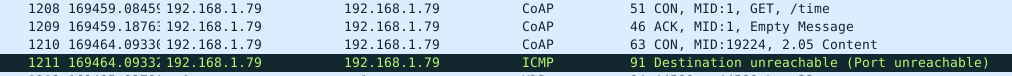
\includegraphics[width=1\columnwidth]{Pictures/get-time1.png}}
\caption{Échange incomplet}
\label{fig-get-time1}
\end{figure}

         \vspace{1em}


\lgf{La solution est d'attendre un second message et de le décoder comme le montre le listing suivant qui donne le code du programme \lprog{coap\_get\_time2.py}{pycom} dans lequel vous n'aurez pas oublié de changer l'adresse IP du serveur.}
\lge{The solution is to wait for a second message and to decode it as shown in the following listing which gives the code of the program \lprog{coap\_get_time2.py}{pycom} in which you will not have forgotten to change the server IP address.}


\pycomlst{coap\_get\_time2.py}

\lgf{Nous pouvons laisser éclater notre joie car nous avons la réponse :}
\lge{We can let our joy explode because we have the answer:}


\begin{termc}[backgroundcolor=\color{gray!10}, basicstyle=\ttfamily\small, escapechar=@] 
> python3 coap_get_time2.py
False
CON  0x0001 GET   
> Uri-path : b'time'
ACK  0x0001 EMPTY 
CON  0x2708 2.05  
---CONTENT
hex: b'323032312d30332d33302031343a3537'
txt: b'2021-03-30 14:57'
\end{termc}

\lgf{Mais notre joie est de courte durée car si on regarde plus attentivement la figure~\vref{fig-get-time2} le trafic sur le réseau, on voit que la réponse a été émise deux fois et que l'on retrouve ensuite une erreur ICMP. Cela est dû au fait que l'on n'acquitte pas le message venant du serveur. Le croyant perdu, il le retransmet et tombe sur une socket inexistante.}
\lge{But our joy is short-lived because if we look more closely at the figure~\vref{fig-get-time2} the traffic on the network, we see that the response was sent twice and that we then find an ICMP error. This is due to the fact that the message from the server is not acknowledged. Believing it to be lost, it retransmits it and finds a non-existent socket.}




\begin{figure}[tbp]
\centerline{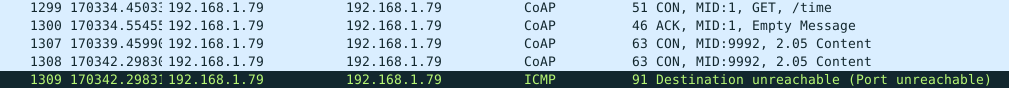
\includegraphics[width=1\columnwidth]{Pictures/get-time2.png}}
\caption{Échange encore incomplet}
\label{fig-get-time2}
\end{figure}

         \vspace{1em}

\lgf{Pour bien faire, nous devons fournir un acquittement au serveur avec ce code de client avec le programme \lprog{coap\_get\_time3.py}{pycom}.}
\lge{To do well, we must provide an acknowledgement to the server with this client code with the program \lprog{coap\_get\_time3.py}{pycom}.}


\pycomlst{coap\_get\_time3.py}

\lgf{Ici, l'exécution est parfaite :}
\lge{Here, the execution is perfect:}


\begin{termc}[backgroundcolor=\color{gray!10}, basicstyle=\ttfamily\small, escapechar=@] 
> python3 coap_get_time3.py
False
CON  0x0001 GET   
> Uri-path : b'time'
ACK  0x0001 EMPTY 
CON  0x2709 2.05  
---CONTENT
hex: b'323032312d30332d33302031353a3133'
txt: b'2021-03-30 15:13'
ACK  0x2709 EMPTY 
\end{termc}

\noindent 
\lgf{si vous n'avez pas oublié de changer l'adresse IP du serveur, et l'utilisation du réseau est optimale (cf figure~\vref{fig-get-time3}).}
\lge{if you did not forget to change the IP address of the server, and the use of the network is optimal (cf figure~\vref{fig-get-time3}).}


\begin{figure}[tbp]
\centerline{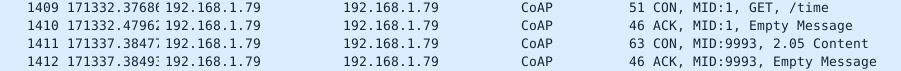
\includegraphics[width=1\columnwidth]{Pictures/get-time3.png}}
\lgf{\caption{Échange dans les règles de l'art}}
\lge{\caption{State of the art exchange}}
\label{fig-get-time3}
\end{figure}

\lgf{Enfin, on peut ajouter un token pour lier les deux transactions. Ici, il n'y a pas d’ambiguïté car nous ne demandons qu'une seule ressource. Mais si nous demandions plusieurs ressources simultanément, il faudrait pouvoir associer la réponse à la requête. Le programme \lprog{coap\_get\_time4.py}{pycom} ajoute lors de la création de l'en-tête un champ token.}
\lge{Finally, we can add a token to link the two transactions. Here, there is no ambiguity because we only request one resource. But if we were to request several resources simultaneously, we would have to be able to associate the response with the request. The program \lprog{coap\_get\_time4.py}{pycom} adds a token field when creating the header.}


\pycomlst[firstline=9,lastline=12, firstnumber=9]{coap\_get\_time4.py}

\lgf{L'échange est le même mais le token est répété dans la réponse.}
\lge{The exchange is the same but the token is repeated in the response.}


\begin{termc}[backgroundcolor=\color{gray!10}, basicstyle=\ttfamily\small, escapechar=@] 
> python3 coap_get_time4.py
False
CON  0x0001 GET   T=012345
> Uri-path : b'time'
ACK  0x0001 EMPTY 
CON  0x270A 2.05  T=012345
---CONTENT
hex: b'323032312d30332d33302031353a3232'
txt: b'2021-03-30 15:22'
ACK  0x270A EMPTY 
\end{termc}

\Question{NON}
{
\lgf{Que se passe-t-il si vous utilisez une requête non confirmable pour demander la ressource /time (mettre l'argument \texttt{type=CoAP.NON} dans la construction de l'en-tête obligatoire).}
\lge{What happens if you use a non-confirmable request to ask for the /time resource (put the argument \texttt{type=CoAP.NON} in the mandatory header construction).}

 \begin{itemize}[label=$\circ$]
   \item \Wrong{
    \lgf{Ça plante le serveur.}
    \lge{The server crashes.}
    }
   \item \Wrong{
    \lgf{Le serveur répond par une requête Confirmable.}
    \lge{The server responds with a Confirmable request.}
    }
   \item \Wrong{ 
    \lgf{Le serveur retourne un RST car nous n'avons pas programmé ce cas.}
    \lge{The server returns an RST because we have not programmed this case.}
    }
   \item \Correct{
    \lgf{Le serveur répond par une requête Non Confirmable.}
    \lge{The server responds with an Unconfirmable request.}
    }
   \item \Wrong{
    \lgf{On passe en heure d'hiver.}
    \lge{We switch to winter time.}
    }
\end{itemize}
}
{}

\Question{\lgf{Réponse immédiate et CON}\lgf{Immediate response and CON}}{
\lgf{Modifiez le programme du serveur pour supprimer le délai de 5 secondes avant une réponse.}
\lge{Modify the server program to remove the 5 second delay before a response.}


\lgf{Que se passe-t-il quand le client envoie une requête CONfirmable ?}
\lge{What happens when the client sends a CONfirmable request?}


 \begin{itemize}[label=$\circ$]
   \item \Correct{
    \lgf{Le serveur retourne la réponse dans l'acquittement.}
    \lge{The server returns the answer in the acknowledgement.}
    }
   \item \Wrong{
    \lgf{Le serveur retourne une requête NON confirmable.}
    \lge{The server returns a NON confirmable request.}
    }
   \item \Wrong{
    \lgf{Le serveur attend quand même quelques secondes pour ne pas saturer le réseau.}
    \lge{The server still waits a few seconds to avoid saturating the network.}
    }
   \item \Wrong{
    \lgf{Le serveur enlève le token de la réponse.}
    \lge{The server removes the token from the response.}
    }
\end{itemize}
 }{}
 
 \Question{\lgf{Réponse immédiate et NON}\lge{Immediate response and NON}}{
\lgf{Modifiez le programme du serveur pour supprimer le délai de 5 secondes avant une réponse.}
\lge{Modify the server program to remove the 5 second delay before a response.}


\lgf{Que se passe-t-il quand le client envoie une requête NON confirmable ?}
\lge{What happens when the client sends a NON confirmable request?}


 \begin{itemize}[label=$\circ$]
   \item \Wrong{
        \lgf{Le serveur retourne la réponse dans l'acquittement.}
        \lge{The server returns the answer in the acknowledgement.}
        }
   \item \Correct{
        \lgf{Le serveur retourne une requête NON confirmable.}
        \lge{The server returns a NON confirmable request.}
        }
   \item \Wrong{
        \lgf{Le serveur attend quand même quelques secondes pour ne pas saturer le réseau.}
        \lge{The server still waits a few seconds to avoid saturating the network.}
        }
   \item \Wrong{
        \lgf{Le serveur enlève le token de la réponse.}
        \lge{The server removes the token from the response.}
        }
\end{itemize}
 }{}
 
 
 \section{POST}
 
 \lgf{\subsection {Ressource codée en ASCII}}
 \lge{\subsection {ASCII encoded resource}}
 
 
\lgf{Nous allons voir le traitement d’une requête POST avec \textit{aiocoap}. Nous aurions pu ajouter ce traitement à la classe \pfunction{aiocoap}{TimeResource} vue précédemment, mais nous avons préféré ajouter une nouvelle ressource pour le traitement des températures.}
\lge{We will see the processing of a POST request with \textit{aiocoap}. We could have added this processing to the \pfunction{aiocoap}{TimeResource} class seen earlier, but we preferred to add a new resource for temperature processing.}


\lgf{Les lignes suivantes ont été ajoutées pour traiter le POST. Notez le nom de la méthode \texttt{render\_post}.}
\lge{The following lines have been added to handle the POST. Note the method name \texttt{render\_post}.}

\pythonlst[firstline=34,lastline=39, firstnumber=34]{coap\_basic\_server2.py}


\lgf{La réponse à la requête est le code 2.04 (\texttt{aiocoap.CHANGED}) qui indique que la ressource été modifiée. }
\lge{The response to the request is code 2.04 (\texttt{aiocoap.CHANGED}) which indicates that the resource was modified. }

\lgf{On lui associe une nouvelle classe dans l’arbre des ressources :}
\lge{It is associated with a new class in the resource tree:}


\pythonnxt[firstline=59,lastline=59, firstnumber=59]{coap\_basic\_server2.py}

\lgf{Le tout forme le programme \pprog{coap\_basic\_server2.py}{plido-tp4}.}
\lge{The whole forms the program \pprog{coap\_basic_server2.py}{plido-tp4}.}


         \vspace{1em}

\lgf{Coté client, le principe est le même que pour le GET. Dans le programme \lprog{coap\_post\_temp1.py}{pycom}, la méthode \pfunction{CoAP}{add\_payload} permet d’ajouter du contenu à la requête POST. Le programme émet sa requête et affiche le résultat. Nous allons également simplifier la gestion des réponses en utilisant la fonction \pfunction{CoAP}{send\_ack} du module \texttt{CoAP}. Cette fonction prend en argument une socket, un tuple de destination et le message CoAP à envoyer. Elle va le retransmettre au maximum 4 fois tant qu’elle n’a pas reçu l’acquittement correspondant.}
\lge{On the client side, the principle is the same as for the GET. In the program \lprog{coap\_post\_temp1.py}{pycom}, the method \pfunction{CoAP}{add\_payload} allows to add content to the POST request. The program sends its request and displays the result. We are also going to simplify the management of the responses by using the function \pfunction{CoAP}{send\_ack} of the module \texttt{CoAP}. This function takes as argument a socket, a destination tuple and the CoAP message to send. It will retransmit it at most 4 times until it has received the corresponding acknowledgement.}

\pycomlst{coap\_post\_temp1.py} %[firstline=9,lastline=12, firstnumber=9]

\lgf{La figure~\vref{fig-duree-max} a montré un échange avec perte. Elles peuvent être simulées en arrêtant le programme serveur sur votre ordinateur.}
\lge{Figure~\vref{fig-duree-max} showed a lossy exchange. They can be simulated by stopping the server program on your computer.}

\lgf{Lancez le serveur \pprog{coap\_basic\_server2.py}{plido-tp4} et tapez ctrl-Z pour stopper son exécution, tout en laissant ouverte la socket.}
\lge{Launch the server \pprog{coap\_basic_server2.py}{plido-tp4} and type ctrl-Z to stop its execution, while leaving the socket open.}

\begin{termc}[backgroundcolor=\color{palerod}, basicstyle=\ttfamily\small, escapechar=@] 
> python3 ./coap_basic_server2.py 
server running on  192.168.1.79 at port 5683 ^Z
Job 2, “python3 ./coap_basic_server2.py” has stopped
>
\end{termc}

\lgf{Lancez le client \lprog{coap\_port\_temp1.py}{pycom} (en n'oubliant pas de changer l'adresse IP du serveur).}
\lge{Launch the client \lprog{coap\_port\_temp1.py}{pycom} (don't forget to change the server IP address).}


\begin{termc}[backgroundcolor=\color{gray!10}, basicstyle=\ttfamily\small, escapechar=@] 
> python3.9 coap_post_temp1.py 
False
CON  0x0001 POST  
> Uri-path : b'temp'
---CONTENT
hex: b'32332e35'
txt: b'23.5'
timeout 2 1
timeout 4 2
\end{termc}

\lgf{On voit que le client ne reçoit pas l'acquittement, déclenche un temporisateur et retransmet le message. La durée du temporisateur double à chaque tentative\footnote{Le standard recommande d'ajouter un aléa lors de la transmission pour éviter que deux équipements se synchronisent et se perturbent toujours en même temps. Il n'est pas mis en œuvre dans cet exemple.}.}
\lge{We see that the client does not receive the acknowledgement, triggers a timer and retransmits the message. The duration of the timer doubles with each attempt\footnote{The standard recommends adding a randomness during the transmission to avoid that two equipments synchronize and disturb each other always at the same time. It is not implemented in this example}.}


\lgf{Réactivez le serveur coap en tapant \texttt{fg} (foregroung)}
\lge{Reactivate the coap server by typing \texttt{fg} (foregroung)}


\begin{termc}[backgroundcolor=\color{palerod}, basicstyle=\ttfamily\tiny, escapechar=@] 
> fg
DEBUG:coap-server:Incoming message <aiocoap.Message at 0x7f05d621fcc0: Type.CON POST (MID 1, empty token) remote 
<UDP6EndpointAddress 192.168.1.79:37286 (locally 192.168.1.79%lo)>, 1 option(s), 4 byte(s) payload>
DEBUG:coap-server:New unique message received
--------------------
payload: b'32332e35'
DEBUG:coap-server:Sending message <aiocoap.Message at 0x7f05d622df98: Type.ACK 2.04 Changed (MID 1, empty token) 
remote <UDP6EndpointAddress 192.168.1.79:37286 (locally 192.168.1.79%lo)>>
DEBUG:coap-server:Incoming message <aiocoap.Message at 0x7f05d621fcc0: Type.CON POST (MID 1, empty token) remote 
<UDP6EndpointAddress 192.168.1.79:37286 (locally 192.168.1.79%lo)>, 1 option(s), 4 byte(s) payload>
INFO:coap-server:@\ul{Duplicate CON received, sending old response again}@
DEBUG:coap-server:Sending message <aiocoap.Message at 0x7f05d622df98: Type.ACK 2.04 Changed (MID 1, empty token) 
remote <UDP6EndpointAddress 192.168.1.79:37286 (locally 192.168.1.79%lo)>>
DEBUG:coap-server:Socket error recevied, details: SockExtendedErr(ee_errno=111, ee_origin=2, ee_type=3, ee_code=3, 
ee_pad=0, ee_info=0, ee_data=0)
DEBUG:coap-server:Incoming error 111 from <UDP6EndpointAddress 192.168.1.79:37286 (locally 192.168.1.79%lo)>
DEBUG:coap-server:Incoming message <aiocoap.Message at 0x7f05d622deb8: Type.CON POST (MID 1, empty token) remote 
<UDP6EndpointAddress 192.168.1.79:37286 (locally 192.168.1.79%lo)>, 1 option(s), 4 byte(s) payload>
INFO:coap-server:@\ul{Duplicate CON received, sending old response again}@
DEBUG:coap-server:Sending message <aiocoap.Message at 0x7f05d622df98: Type.ACK 2.04 Changed (MID 1, empty token) 
remote <UDP6EndpointAddress 192.168.1.79:37286 (locally 192.168.1.79%lo)>>
DEBUG:coap-server:Socket error recevied, details: SockExtendedErr(ee_errno=111, ee_origin=2, ee_type=3, ee_code=3, 
ee_pad=0, ee_info=0, ee_data=0)
DEBUG:coap-server:Incoming error 111 from <UDP6EndpointAddress 192.168.1.79:37286 (locally 192.168.1.79%lo)>
\end{termc}

\lgf{On peut observer plusieurs phénomènes :}
\lge{Several phenomena may be observed:}


\begin{itemize}
    \item 
        \lgf{le serveur avait gardé en mémoire les requêtes précédentes mais ne les avait pas traitées car le programme avait été stoppé. En le redémarrant, il va pouvoir les traiter. Il répond donc au client qui peut afficher la notification 2.04 ;}
        \lge{the server had kept in memory the previous requests but had not processed them because the program had been stopped. By restarting it, it will be able to process them. It then replies to the client, which can display the notification 2.04 ;}
        
    \item 
        \lgf{les autres requêtes sont vues comme des répétitions de la première puisque le champ Message ID est identique. Le serveur se contente de retourner une copie ;}
        \lge{the other requests are seen as repeats of the first one since the Message ID field is identical. The server simply returns a copy;}
        
    \item 
        \lgf{le client ayant terminé sa transaction a fermé la socket conduisant à l'émission d'un message ICMP qui conduit à l'affichage du message de log d'erreur (Socket error received). }
        \lge{the client having finished its transaction has closed the socket leading to the emission of an ICMP message which leads to the display of the error log message (Socket error received). }
        
\end{itemize}

         \vspace{1em}


\lgf{Ceci peut être vérifié sur la capture Wireshark (cf. figure~\vref{fig-post-ws}).}
\lge{This can be verified on the Wireshark capture (see figure~\vref{fig-post-ws}).}


\begin{figure}[tbp]
\centerline{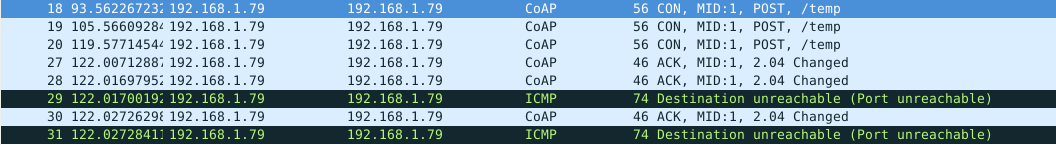
\includegraphics[width=1\columnwidth]{Pictures/coap-ws.png}}
\lgf{\caption{Trafic lié au POST}}
\lge{\caption{POST related traffic}}

\label{fig-post-ws}
\end{figure}


\lgf{\subsection{Ressource codée en CBOR}}
\lge{\subsection{Resource coded in CBOR}}

\lgf{Le programme précédent, est correct mais nous avons utilisé le format ASCII de transfert par défaut (\textit{\Index{Content-format}} = 0). Il serait préférable de revenir au format JSON ou \Index{CBOR} que nous avions vu précédemment. Pour ce faire, nous devons ajouter dans l’en-tête de la requête l’option Content-format. Comme son code est 12, elle doit être placée après l’option Uri-path (cf. tableau~\vref{tab-CoAP-options}).}
\lge{The previous program is correct but we used the default ASCII transfer format (\textit{\Index{Content-format}} = 0). It would be better to return to the JSON or \Index{CBOR} format that we had seen previously. To do this, we must add the Content-format option to the request header. As its code is 12, it must be placed after the Uri-path option (see table~\vref{tab-CoAP-options}).}


\pycomlst{coap\_post\_temp2.py} %[firstline=9,lastline=12, firstnumber=9]

\lgf{Notez que ce programme,  pprog{coap\_post\_temp2.py}{pycom},  peut aussi bien s'exécuter sur votre ordinateur ou sur votre LoPy. Dans le premier cas, le module \texttt{cbor2} sera utilisé. Sur le LoPy, nous ferons appel au module \texttt{kpn\_senml}. Dans les deux cas, le contenu est transformé en CBOR grâce à la fonction \pfunction{cbor2}{dumps}.}
\lge{Note that this program, pprog{coap\_post\_temp2.py}{pycom}, can be run on your computer or on your LoPy. In the first case, the module \texttt{cbor2} will be used. On the LoPy, we will use the module \texttt{kpn\_senml}. In both cases, the content is transformed into CBOR thanks to the function \pfunction{cbor2}{dumps}.}


         \vspace{1em}

\lgf{Du coté du serveur, la méthode\texttt{render\_post} doit connaître le format de la ressource. Pour ce faire, elle doit accéder aux options CoAP.}
\lge{On the server side, the methodtexttt{render\_post} must know the format of the resource. To do this, it must access the CoAP options.}


\pythonlst[firstline=34,lastline=50, firstnumber=34]{coap\_basic\_server3.py} %

\lgf{Dans le programme \pprog{coap\_basic\_server3.py}{plido-tp4}, la variable \texttt{ct} contient la valeur de l’option \Index{Content-format} si elle existe. De manière générale, \textit{aiocoap} permet d’accéder aux valeurs de toutes les options CoAP contenues dans la requête. La valeur \texttt{None} indique que l’option n’est pas présente dans l’en-tête. Dans ce cas, la variable \texttt{ct} contiendra la valeur par défaut indiquant un texte en ASCII.}
\lge{In the program \pprog{coap\_basic\_server3.py}{plido-tp4}, the variable \texttt{ct} contains the value of the option \Index{Content-format} if it exists. In general, \textit{aiocoap} allows access to the values of all CoAP options contained in the request. The value \texttt{None} indicates that the option is not present in the header. In this case, the variable \texttt{ct} will contain the default value indicating ASCII text.}


\lgf{Suivant le format de la donnée, le programme affichera le texte ou le CBOR transformé en chaîne de caractères avec la fonction \pfunction{cbor2}{loads}. Si le format n’est pas connu du programme, un code d’erreur est retourné au client.}
\lge{Depending on the format of the data, the program will display the text or the CBOR transformed into a character string with the function \pfunction{cbor2}{loads}. If the format is not known to the program, an error code is returned to the client.}


         \vspace{1em}

\lgf{La figure~\vref{fig-post2-ws} montre l'échange lié au POST et détaille contenu de la requête.}
\lge{The figure~\vref{fig-post2-ws} shows the exchange related to the POST and details the content of the request.}


\begin{figure}[tbp]
\centerline{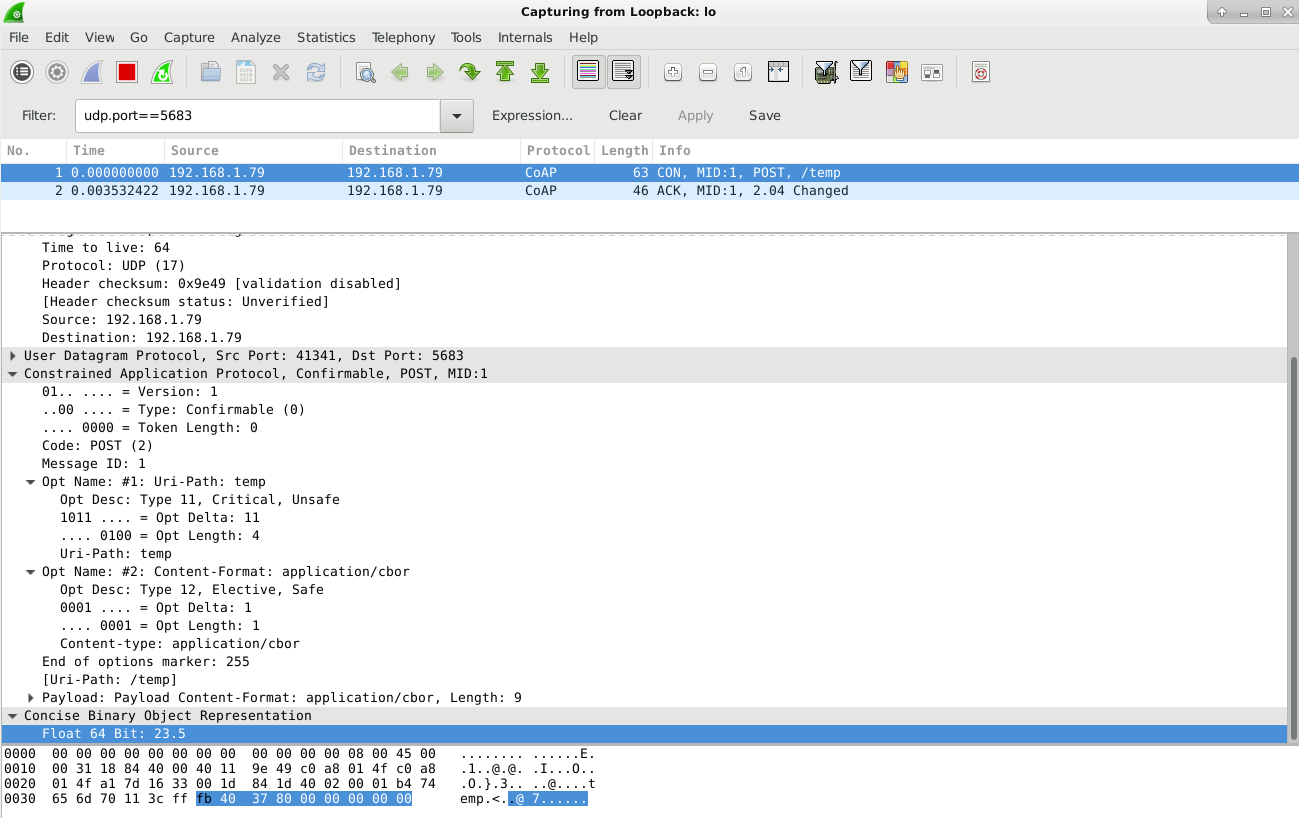
\includegraphics[width=1\columnwidth]{Pictures/aiocoap-ws.png}}
\lgf{\caption{Trafic complet lié au POST}}
\lge{\caption{Full POST traffic}}
\label{fig-post2-ws}
\end{figure}

\Question{\lgf{Réponse}\lge{Response}}
{
\lgf{Que reçoit-on en réponse à la requête POST ?}
\lge{What do we receive in response to the POST request?}

 \begin{itemize}[label=$\circ$]
   \item \Wrong{
    \lgf{un message ACK}
    \lge{an ACK message}
    }
   \item \Wrong{
    \lgf{le statut 2.00 OK.}
    \lge{status 2.00 OK.}
    }
   \item \Correct{
    \lgf{le statut 2.04 CHANGED.}
    \lge{status 2.04 CHANGED.}
    }
   \item \Wrong{
    \lgf{rien.}
    \lge{nothing.}
    }
\end{itemize}
 }
{
\lgf{A chaque requête on reçoit une notification REST indiquant que la ressource a été modifiée. }
\lge{At each request we receive a REST notification indicating that the resource has been modified. }
}

\Question{JSON}
{
\lgf{Modifiez le programme client pour indiquer un content-format JSON. Quelle notification obtenez-vous ?}
\lge{Modify the client program to specify a JSON content-format. What notification do you get?}

 \begin{itemize}[label=$\circ$]
   \item \Wrong{
    \lgf{un message RST}
    \lge{an RST message}
    }
   \item \Wrong{
    \lgf{le statut 4.04 NOT FOUND.}
    \lge{le statut 4.04 NOT FOUND.}
    }
   \item \Correct{
    \lgf{le statut 2.15.}
    \lge{le statut 2.15.}
    }
   \item \Wrong{
    \lgf{le statut 5.00.}
    \lge{statut 5.00.}
    }
\end{itemize}
 }
{
\lgf{Si vous avez 5.00 c'est qu'il y a une erreur dans votre programme coté serveur. La notification pour un format inconnu est 4.15 (Unsupported Content-Format)}
\lgf{If you have 5.00 it means that there is an error in your server side program. The notification for an unknown format is 4.15 (Unsupported Content-Format)}

}

\subsection{No Response}

\lgf{Que l'on utilise le type CONfirmable ou NON confirmable, le serveur va envoyer une notification : }
\lge{Whether you use the CONfirmable or NON-confirmable type, the server will send a notification : }

\begin{itemize}
\item 
    \lgf{2.xx quand tout se passe bien, et}
    \lge{2.xx when everything is going well, and}
\item
    \lgf{4.xx ou 5.xx quand le client ou le serveur a commis une erreur.}
    \lge{4.xx or 5.xx when the client or server has made an error.}
\end{itemize}

\lgf{Si un capteur veut utiliser CoAP sur un réseau LPWAN, à chaque POST qu'il va envoyer sur la voie montante (uplink), il va récupérer un acquittement dans la voie descendante (downlink). Or, on a vu que l'on devait ménager cette dernière qui pouvait être sujette à saturation ou à facturation. }
\lge{If a sensor wants to use CoAP on an LPWAN network, for each POST it sends on the uplink, it will get an acknowledgement in the downlink. However, we have seen that we must be careful with the downlink channel, which could be subject to saturation or billing. }

\lgf{L'option \Index{No response} définie dans le RFC 7967 permet à un client d'informer le serveur qu'il ne souhaite pas recevoir de notifications lors d'un POST ou d'un PUT.  La valeur de l'option est 258 et elle est suivie d'un octet contenant un bitmap qui va indiquer quel type de notification va être émis :}
\lge{The \Index{No response} option defined in RFC 7967 allows a client to inform the server that it does not wish to receive notifications during a POST or PUT.  The value of the option is 258 and it is followed by a byte containing a bitmap that will indicate what type of notification will be sent:}

\begin{itemize}
    \item 
        \lgf{si le deuxième bit à partir de la droite est mis à 1, le client ne veut pas recevoir les notifications de type 2.xx ;}
        \lge{if the second bit from the right is set to 1, the client does not want to receive notifications of type 2.xx ;}
        
    \item 
        \lgf{si le quatrième bit à partir de la droite est mis à 1, le client ne veut pas recevoir les notifications de type 4.xx ;}
        \lge{if the fourth bit from the right is set to 1, the client does not want to receive notifications of type 4.xx ;}
        
    \item 
        \lgf{si le cinquième bit à partir de la droite est mis à 1, le client ne veut pas recevoir les notifications de type 5.xx.}
        \lge{if the fifth bit from the right is set to 1, the client does not want to receive notifications of type 5.xx.}
\end{itemize}

\lgf{Par exemple, en mettant la valeur \texttt{0x02} dans cette option, le client ne reçoit pas les acquittements positifs mais uniquement les erreurs 4.xx et 5.xx. En mettant la valeur \texttt{0b00011010} (0x1a, 26), le serveur sera complètement silencieux.}
\lge{For example, by setting the value \texttt{0x02} in this option, the client does not receive positive acknowledgements but only errors 4.xx and 5.xx. By setting the value \texttt{0b00011010} (0x1a, 26), the server will be completely silent.}

\lgf{Le programme \pprog{coap\_post\_temp4.py}{pycom} ajoute cette option et le type du message CoAP a été fixé à NON confirmable. Cependant, le chemin d'URI n'est pas connu du serveur.  On voit que le serveur retourne un message d'erreur. Si en revanche le POST se déroule correctement, seul le client émet une donnée et le serveur reste silencieux.}
\lge{The program \pprog{coap\_post\_temp4.py}{pycom} adds this option and the type of the CoAP message has been set to NOT confirmable. However, the URI path is not known to the server.  We see that the server returns an error message. If, on the other hand, the POST is successful, only the client sends data and the server remains silent.}


\pycomlst[firstline=15,lastline=21, firstnumber=15]{coap\_post\_temp4.py}

\lgf{\section{Chaîne complète de remonté de mesures}}
\lge{\section{Complete chain of measurements}}


 \begin{wrapfigure}{r}{3cm}
\Youtube{https://youtu.be/TFeeSEqGhPk}
\end{wrapfigure}


\lgf{Voilà ! nous pouvons mettre les différents concepts ensemble pour construire une chaîne complète de remontée d'informations sur la température, l'humidité et la pression.}
\lge{Voilà !  Now we can put the different concepts together to build a complete feedback chain for temperature, humidity and pressure.}


         \vspace{1em}

\lgf{Côté capteur, nous allons~:}
\lge{On the sensor side, we will~:}

\begin{itemize}
    \item 
        \lgf{si le BME280 est présent, récupérer directement les données. Sinon, nous allons utiliser les mesures virtuelles. Nous allons également définir le protocole réseau : WiFi, Sigfox, LoRaWAN ;}
        \lge{if the BME280 is present, retrieve the data directly. Otherwise, we will use virtual measurements. We will also define the network protocol: WiFi, Sigfox, LoRaWAN;}
    \item 
        \lgf{si nous utilisons un réseau LoRaWAN, nous devons mettre en place un programme relais pour transmettre les données vers le serveur CoAP ;}
        \lge{if we use a LoRaWAN network, we have to set up a relay program to transmit the data to the CoAP server;}
\end{itemize}

\lgf{Le serveur CoAP doit pouvoir envoyer les données au serveur Beebotte pour affichage.}
\lge{The CoAP server must be able to send the data to the Beebotte server for display.}

         \vspace{1em}

\lgf{Le message CoAP va être configuré de la manière suivante :}
\lge{The CoAP message will be configured as follows:}

\begin{itemize}
\item 
    \lgf{type = NON pour éviter les acquittements des messages CoAP ;}
    \lgf{type = NON to avoid acknowledgements of CoAP messages;}
    
\item 
    \lgf{l'option No Response à 2 pour éviter les notifications REST positives. On garde sur la voie descendante les notifications d'erreurs pour permettre au capteur d'arrêter de transmettre ou d'augmenter sa période d'émission si le serveur n'est pas capable de traiter les données. Cela permettra de limiter l'usage du spectre et de préserver l'énergie des capteurs ;}
    \lgf{the No Response option to 2 to avoid positive REST notifications. Error notifications are kept on the downstream channel to allow the sensor to stop transmitting or to increase its transmission period if the server is not able to process the data. This will limit the use of the spectrum and preserve the energy of the sensors;}
    
\item 
    \lgf{3 chemins d'URI pour les 3 valeurs mesurées ;}
    \lgf{3 URI paths for the 3 measured values;}
    
\item  
    \lgf{le codage en CBOR des séries temporelles.}
    \lgf{CBOR coding of time series.}
\end{itemize}

         \vspace{1em}

\lgf{Il reste un point à traiter car avec la limitation à 12 octets des trames \Index{Sigfox}, il est impossible de transmettre des données si on utilise CoAP. En effet, l'en-tête CoAP va contenir :}
\lge{There is still a point to be dealt with because with the 12 bytes limitation of the frames \Index{Sigfox}, it is impossible to transmit data if one uses CoAP. Indeed, the CoAP header will contain:}

\begin{itemize}
\item 
    \lgf{4 octets pour l'en-tête obligatoire ;}
    \lge{4 bytes for the mandatory header ;}
\item  
    \lgf{0 octets de Token ;}
    \lge{0 Token bytes ;}
\item  
    \lgf{2 octets au minimum pour l'option URI-path si on réduit à un caractère le chemin ; par exemple \texttt{T}, \texttt{H}, \texttt{P} pour représenter la température, l'humidité et la pression ;}
    \lge{2 bytes minimum for the URI-path option if the path is reduced to one character; for example \texttt{T}, \texttt{H}, \texttt{P} to represent temperature, humidity and pressure;}
\item  
    \lgf{2 octets pour l'option \Index{Content-format} indispensable pour indiquer que l'on transporte du CBOR ;}
    \lge{2 bytes for the option \Index{Content-format} necessary to indicate that one carries CBOR;}
\item  
    \lgf{3 octets pour l'option \Index{No-response}, également indispensable pour indiquer que l'on ne veut surtout pas d'acquittement (Sigfox les limitant à 4 par jour).}
    \lge{3 bytes for the option \Index{No-response}, also essential to indicate that we do not want any acknowledgement (Sigfox limiting them to 4 per day).}
\end{itemize}

\lgf{Soit, au total 11 octets. Il n'en reste plus qu'un. Si la température dépasse les 23 °C, l'information ne sera pas transportable.}
\lge{That is, a total of 11 bytes. There is only one left. If the temperature exceeds 23°C, the information will not be transportable.}


\section{SCHC}

\lgf{\acl{SCHC}, défini dans le \rfc{8724}, donne l'acronyme SCHC que l'on prononce Chic. SCHC propose un mécanisme de compression générique des en-têtes. SCHC se base sur un contexte commun à l'émetteur et au récepteur qui va permettre d'éliminer les informations connues dans le message et de ne transmettre que les données qui ne peuvent pas être prédéterminées.}
\lge{\acl{SCHC}, defined in the \rfc{8724}, gives the acronym SCHC which we pronounce Chic. SCHC proposes a generic compression mechanism for headers. SCHC is based on a context common to the sender and the receiver which will make it possible to eliminate the known information in the message and to transmit only the data which cannot be predetermined.}


         \vspace{1em}

\lgf{Nous allons mettre en œuvre une version simplifiée. Dans le message CoAP, nous avons besoin du champ Message ID qui va servir à éliminer les doublons qui pourraient apparaître dans le réseau. Les serveurs CoAP gardent en mémoire les informations concernant les Messages ID pendant 5 minutes. Donc, la numérotation des messages doit permettre des périodes plus longues avant de réutiliser les mêmes valeurs. Nous allons également transporter 3 types de ressources : \texttt{/temperature}, \texttt{/humidity} et \texttt{/pressure}.}
\lge{We will implement a simplified version. In the CoAP message, we need the Message ID field that will be used to eliminate duplicates that might appear in the network. The CoAP servers keep the information about the Message IDs in memory for 5 minutes. Therefore, the message numbering must allow for longer periods before reusing the same values. We will also carry 3 types of resources: \texttt{/temperature}, \texttt{/humidity} and \texttt{/pressure}.}


         \vspace{1em}

\lgf{On peut donc construire manuellement un en-tête SCHC avec les champs suivants :}
\lge{We can therefore manually build a SCHC header with the following fields:}

\begin{itemize}
\item 
    \lgf{2 bits pour numéroter les règles de compression. Dans notre cas, nous n'utiliserons que la règle 00 ;}
    \lge{2 bits to number the compression rules. In our case, we will only use rule 00 ;}
    
\item 
    \lgf{4 bits pour numéroter les messages ID, ce qui donne 15 valeurs possibles de 1 à 15. Au pire, il faudrait émettre plus de 3 trames par minutes pour que le serveur CoAP traite deux trames différentes comme des doublons ;}
    \lge{4 bits to number the ID messages, which gives 15 possible values from 1 to 15. In the worst case, more than 3 frames per minute would have to be transmitted for the CoAP server to treat two different frames as duplicates;}
    
\item 
    \lgf{2 bits pour désigner les chemins d'URI ; 3 seront utilisés.}
    \lge{2 bits to designate URI paths; 3 will be used.}
    
\end{itemize}

         \vspace{1em}

\lgf{Cela fait appel à plusieurs techniques de compression définies par SCHC :}
\lge{This involves several compression techniques defined by SCHC:}

\begin{itemize}
\item 
    \lgf{\textit{\Index{not\_sent}}~: la valeur d'un champ n'est pas envoyée sur le réseau car elle se trouve dans les règles. Cela s'appliquera à la plupart des champs ;}
    \lge{\textit{\Index{not\_sent}}~: the value of a field is not sent on the network because it is in the rules. This will apply to most fields;}
    
    
\item 
    \lgf{\textit{\Index{Least Significant Bit}} : on n'envoie que les bits de poids faible. Cela s'applique au champ Message ID duquel on ne va transmettre que les 4 bits de poids faible ;}
    \lge{\textit{\Index{Least Significant Bit}} : only the least significant bits are sent. This applies to the Message ID field, for which only the 4 least significant bits will be transmitted;}
    
\item 
    \lgf{\textit{\Index{Matching\_sent}} : au lieu d'envoyer la valeur, on va envoyer un index sur un tableau commun. Cela s'applique à Uri-path où l'on enverra 00 pour l'élément temperature, 01 pour l'élément pressure, et 10 pour élément humidity. }
    \lge{\textit{\Index{Matching\_sent}} : instead of sending the value, we will send an index on a common array. This applies to Uri-path where we will send 00 for the temperature element, 01 for the pressure element, and 10 for the humidity element. }
    
\end{itemize}

         \vspace{1em}

\lgf{\subsection{Emission côté client}}
\lge{\subsection{Client-side transmission}}

\lgf{La compression très simplifiée que nous allons effectuer se fera au moment de l'envoi des données pour Sigfox dans le programme \lprog{coap\_full\_sensor.py}{pycom}.}
\lge{The very simplified compression that we will carry out will be done at the time of the sending of the data for Sigfox in the program \lprog{coap\_full\_sensor.py}{pycom}.}


\pycomlst[firstline=174,lastline=198, firstnumber=174]{coap\_full\_sensor.py}

\lgf{Dans le cas de Sigfox, on prend l'index en cherchant l'élément dans le tableau (ligne 183). On construit ensuite l'octet SCHC en ajoutant un numéro de règle (ligne 185) et les 4 bits de poids faible du champ Message ID qui va donc varier de 1 à 15 (ligne 186). Puis, l'on concatène les données CBOR a envoyer (ligne 193).}
\lge{In the case of Sigfox, one takes the index by seeking the element in the table (line 183). One builds then the byte SCHC by adding a number of rule (line 185) and the 4 bits of low weight of the field Message ID which will thus vary from 1 to 15 (line 186). Then, one concatenates the CBOR data to be sent (line 193).}


         \vspace{1em}

\lgf{Pour les autres technologies de transmission, l'en-tête CoAP est construite avec les fonctions du module CoAP.py.}
\lge{For other transmission technologies, the CoAP header is built with the functions of the CoAP.py module.}


\pycomnxt[firstline=200,lastline=208, firstnumber=200]{coap\_full\_sensor.py}

\lgf{L'envoi de la trame se fait avec la fonction \texttt{send\_ack}. Comme le message est de type NON, cette fonction n'attend pas de réponse après l'émission des données.}
\lge{The sending of the frame is done with the function \texttt{send\_ack}. As the message is of type NO, this function does not wait for a response after the data is sent.}


\lgf{\subsection{Réception côté serveur}}
\lge{\subsection{Server side reception}}


\lgf{Si les données émises par \lprog{coap\_full\_sensor.py}{pycom} passent par un réseau LPWAN, le programme \pprog{generic\_coap\_relay.py}{plido-tp4} va servir d'intermédiaire pour les envoyer au serveur CoAP. Le programme est presque identique à celui que nous avions utilisé pour transmettre dans la session précédente. Les seules différences sont~:}
\lge{If the data sent by \lprog{coap\_full\_sensor.py}{pycom} passes through an LPWAN network, the program \lprog{generic\_coap\_relay.py}{plido-tp4} will act as an intermediary to send it to the CoAP server. The program is almost identical to the one we used to transmit in the previous session. The only differences are~:}

\begin{itemize}
    \item 
        \lgf{les numéros de ports utilisés : 5683 au lieu de 33033~;}
        \lge{the port numbers used: 5683 instead of 33033~;}
        
    \item 
        \lgf{l'ajout de la décompression SCHC pour les données venant de Sigfox.}
        \lge{the addition of SCHC decompression for data coming from Sigfox.}
        
\end{itemize}

\pythonlst[firstline=69,lastline=89, firstnumber=69]{generic\_coap\_relay.py}

\lgf{Pour reconstruire l'en-tête CoAP, SCHC se base sur des règles pour rendre le traitement indépendant des champs employés par le protocole. Mais ici, pour faire plus simple, nous utilisons le module Message d'\Index{aoicoap} pour reconstituer le message CoAP.}
\lge{To reconstruct the CoAP header, SCHC relies on rules to make the processing independent of the fields used by the protocol. But here, to make it simpler, we use the Message module of \Index{aoicoap} to reconstruct the CoAP message.}


\lgf{Dans un premier temps, on extrait du premier octet la valeur du champ message ID et l'index des URI (ligne 72 à 74) puis, à partir de ces valeurs et de celles connues à l'avance, le message CoAP est reconstitué.}
\lge{Initially, one extracts from the first byte the value of the field message ID and the index of the URI (line 72 to 74) then, starting from these values and those known in advance, the CoAP message is reconstituted.}


         \vspace{1em}

\lgf{Dans tous les cas, la fonction \texttt{forward\_data} est utilisée. Elle retourne la réponse du serveur CoAP qui est renvoyée au réseau LPWAN suivant les principes que nous avions vus lors de la session précédente. Nous ne l'avons pas mis en œuvre pour Sigfox pour éviter une erreur vu que 4 messages par jours sont autorisés.}
\lge{In all cases, the function \texttt{forward\_data} is used. It returns the answer of the CoAP server which is sent back to the LPWAN network according to the principles we had seen during the previous session. We did not implement it for Sigfox to avoid an error since 4 messages per day are allowed.}


\lgf{\subsection{serveur CoAP}}
\lge{\subsection{CoAP server}}


\lgf{Finalement, le programme \pprog{coap\_server.py}{plido-tp4} a été étendu à différents chemins d'URI pour traiter les différentes ressources que vont nous envoyer les capteurs. Et dans le traitement de la ressource, l'appel a la fonction \texttt{to\_bbt} a été ajouté.}
\lge{Finally, the program \pprog{coap\_server.py}{plido-tp4} has been extended to different URI paths to process the different resources that the sensors will send us. And in the treatment of the resource, the call to the function \texttt{to\_bbt} was added.}


\section {Pistes d'améliorations}

\lgf{Vous pouvez étendre cet ensemble de programmes. Voici quelques pistes d'amélioration :}
\lge{You can extend this set of programs. Here are some ways to improve:}


\begin{itemize}

\item 
    \lgf{les capteurs envoient également leur mémoire disponible. Cela peut être utile pour détecter une fuite dans la mémoire ; par exemple quand une structure n'est jamais libérée. La structure CBOR est bien envoyée mais ni \texttt{coap\_server.py} ni Beebotte n'ont été configurés pour afficher ces valeurs. Vous pouvez donc l'intégrer dans la chaîne de traitement ;}
    \lge{sensors also send their available memory. This can be useful to detect a memory leak; for example when a structure is never released. The CBOR structure is sent but neither \texttt{coap\_server.py} nor Beebotte have been configured to display these values. You can therefore integrate it into the processing chain;}
\item 
    \lgf{le POST de la mémoire conduit à l'émission d'un message en downlink pour indiquer l'erreur 4.04. C'est une conséquence de l'utilisation de l'option CoAP \Index{no\_response} qui ne bloque que les notifications de type 2.xx. Vous pouvez modifier le module CoAP.py pour que la réponse soit traitée. Par exemple, en limitant à un envoi par jour de cette ressource ;}
    \lge{the POST from memory leads to a downlink message to indicate error 4.04. This is a consequence of using the CoAP option \Index{no\_response} which only blocks notifications of type 2.xx. You can modify the CoAP.py module so that the response is processed. For example, by limiting this resource to one submission per day;}
\item 
    \lgf{en plus de la mémoire, il peut être intéressant d'envoyer le niveau de la batterie. La page \href{https://forum.pycom.io/topic/1690/correct-formula-for-batt-monitoring-on-expansion-board}{Correct formula for BATT monitoring on expansion board | Pycom user forum}\footnote{https://forum.pycom.io/topic/1690/correct-formula-for-batt-monitoring-on-expansion-board} donne des indications pour récupérer le niveau de la batterie ;}
    \lge{In addition to the memory, it may be interesting to send the battery level. The page \href{https://forum.pycom.io/topic/1690/correct-formula-for-batt-monitoring-on-expansion-board}{Correct formula for BATT monitoring on expansion board | Pycom user forum}\footnote{https://forum.pycom.io/topic/1690/correct-formula-for-batt-monitoring-on-expansion-board} gives indications to recover the battery level;}
\item 
    \lgf{finalement, nous n'avons pas réglé tous les problèmes d'interopérabilité. Si, par exemple, vous voulez envoyer toutes les heures un relevé de la mémoire libre et toutes les minutes la température, vous devez également modifier le programme \texttt{coap\_server.py}. Si ces paramètres sont transmis de manière optimale par le serveur, le programme \texttt{coap\_serveur} peut devenir complètement indépendant de la valeur mesurée.}
    \lge{Finally, we did not solve all the interoperability problems. If, for example, you want to send every hour a reading of the free memory and every minute the temperature, you must also modify the program \texttt{coap\_server.py}. If these parameters are transmitted optimally by the server, the program \texttt{coap\_server} can become completely independent of the measured value.}
\end{itemize}
\Input{Part11.0-LwM2M}






%%%%%%%%%%%%%%%%%%%%%%%%%%%%%%%%%%%%%



\immediate\closeout\tempfile
\setboolean{Response}{false}

\cleardoublepage
\lgf{\chapter{Réponses aux questions}}
\lge{\chapter{Answers to the questions}}
\input{questions}

\cleardoublepage
\printindex

\cleardoublepage
\printbibliography

\end{document}